% Information Processing and Management -- DysLex-Probe
% Ported verbatim from the ESWA submission (ESWA_2026/human_version.tex).
% Body text is UNCHANGED; only the \journal target differs. Abstract to be revised.
% Build with XeLaTeX (Bangla glyphs need fontspec): xelatex main.tex (run 2-3x)
% NOTE: no em-dashes anywhere in rendered text; use -- (en-dash) or rewrite.
\documentclass[preprint,12pt]{elsarticle}

\usepackage{fontspec}
\setmainfont{TeX Gyre Termes}
% Bengali font is bundled in fonts/ so the project also builds on Overleaf,
% where Noto Serif Bengali is not installed as a system font.
\newfontfamily\banglafont[Script=Bengali, Path=fonts/, Extension=.ttf,
  UprightFont=*-Regular, BoldFont=*-Bold]{NotoSerifBengali}
\newcommand{\bn}[1]{{\banglafont #1}}

\usepackage{amsmath,amssymb}
\usepackage{booktabs}
\usepackage{array}
\usepackage{multirow}
\usepackage{graphicx}
\graphicspath{{figs/}}
\usepackage{float}
\usepackage{url}
\usepackage[hidelinks]{hyperref}

% Float placement: keep figures near their references instead of flushing them to the end.
\renewcommand{\topfraction}{0.9}
\renewcommand{\bottomfraction}{0.85}
\renewcommand{\textfraction}{0.08}
\renewcommand{\floatpagefraction}{0.75}
\setcounter{topnumber}{3}
\setcounter{totalnumber}{5}

% Small padding between a (top) table caption and the table body.
\setlength{\belowcaptionskip}{6pt}

% Let TeX stretch interword spacing rather than push text into the margin.
\emergencystretch=3em

\journal{Information Processing and Management}

\begin{document}

\begin{frontmatter}

\title{Surface-controlled cross-lingual probing of multilingual language models for low-resource Bangla dyslexia screening: the roles of tokenization, transfer and localization}

\author[bracu]{Ayesha Siddika\corref{cor1}}
\author[bracu]{Nazmoon Nahar Aka}
\author[bracu]{Mashrafi Rahman}
\author[bracu]{Hasan Mohammad Sayem}
\author[bracu]{Md.\ Tanzim Reza}
\author[bracu]{Farig Yousuf Sadeque}

\affiliation[bracu]{organization={Department of Computer Science and Engineering, BRAC University},
                    city={Dhaka},
                    country={Bangladesh}}

\cortext[cor1]{Corresponding author}

\begin{abstract}
Dyslexia screening in low resource languages is difficult because there are not enough expert clinicians, validated test batteries, or labelled datasets. Multilingual large language models (LLMs) could help as expert systems, but we still do not know which architectures hold lexical information that transfers from a high resource language like English to a low resource one like Bangla, where it is stored, or how tokenization affects it. We probed five publicly available multilingual LLMs -- XLM-RoBERTa large, Llama~3.1 8B, BLOOM 7B1, mT5 XL and ByT5 XL -- with frozen, per layer linear probes on a set of 440 English and Bangla items, reporting bootstrap confidence intervals throughout. After controlling for the first character, character level statistics, and word length, three of four standard phonological probing tasks failed, and only telling real words from pseudowords still worked. On zero-shot transfer to Bangla, BLOOM and ByT5 both reached 0.92 F1 (95\% CI [0.84, 0.98]) and XLM-R 0.86, while Llama (0.63) and mT5 (0.60) dropped to the surface baseline. ByT5 and mT5 share design and training objective and differ mainly in how they break text into units, so ByT5's 0.32 F1 advantage (95\% CI [0.15, 0.49]) shows that tokenization, not the encoder-decoder objective, caused mT5's collapse. Causal ablation also showed a double dissociation: subword encoder models localized the transferable signal, while byte level and decoder models spread it more widely. Finally, a classifier trained on English and tested on Bangla transferred categorical lexical structure above the surface baseline, especially with byte level tokenization, but not abstract, graded item properties. Cross lingual lexical transfer therefore depends mainly on pretraining coverage, the training objective, and tokenization, not on the number of parameters.
\end{abstract}

\begin{keyword}
multilingual language models \sep cross-lingual transfer \sep probing classifiers \sep dyslexia screening \sep low-resource Bangla NLP \sep tokenization \sep mechanistic interpretability \sep bootstrap confidence intervals
\end{keyword}

\end{frontmatter}

% ===========================================================================
\section{Introduction}
\label{sec:intro}
Developmental dyslexia is a specific learning difficulty that affects someone's ability to read words accurately and fluently, decode words, and spell them correctly. These difficulties can occur even when the person has adequate intelligence, schooling, and sensory abilities \cite{snowling2020dyslexia,peterson2012developmental}. It is estimated that dyslexia affects around five to twelve percent of school age children. But this rate changes depending on the language and writing system \cite{ziegler2005reading,wagner2020prevalence}. The most widely accepted explanation for dyslexia is the phonological deficit hypothesis. It suggests that people with dyslexia find it more difficult to represent, remember, and work with speech sounds.
This makes it harder and slower for them to connect written letters, or graphemes, with their corresponding sounds, or phonemes, while learning to read \cite{snowling2020dyslexia,goswami2011temporal}.
The clinical identification of dyslexia usually depends on standard tests designed for a specific language, for example the CTOPP-2 \cite{wagner2013ctopp}. However, these test batteries must be carried out by trained psychometricians, and similar tests are not available for most languages around the world.

More than 270 million people speak Bangla. But it still does not have a widely used, standardised dyslexia screening tool or a fixed diagnostic test battery \cite{nag2014dyslexia,nag2017indian,badsha2024mall}. Because of this people who may have dyslexia are often identified very late or are not identified at all. The lack of these standardised systems creates a major problem to identify dyslexia. It is one of the main reasons for carrying out this research.
At the same time, multilingual LLMs have reached a level where their hidden representations contain detailed linguistic information. This information can be transferred across the languages included in their pretraining data \cite{conneau2020xlmr,scao2022bloom,xue2021mt5}. These models are commonly used for works like translation and dialogue. However as a result of their training they also learn lexical and sublexical information. These are the structures of words and smaller units within words that clinical screening tools are specifically designed to test.
If this information can transfer from a high resource language like English, where validated tests and labelled data are available and to a low resource language like Bangla, where these resources are not available much. One multilingual model can support the development of expert screening prototypes for many languages at the same time. A true phonological representation should work across languages with different levels of orthographic depth. This means differences in how closely letters match sounds. In comparison, representations based only on surface level statistics should not transfer in the same way.

There are, however, three major difficulties to be overcome before an idea like this can be realized as a practical expert system. First, much of the previous probing research employs stimuli that are not appropriately matched. This means that the factors of the surface such as number of characters, number of bytes etc.\ and the type of the initial character is not under control. A probe that is found to recognize voicing might be learning just the first phoneme of the word, so as to not be drawn into phonological learning.
Second, the previous studies report only single point estimates and don't provide confidence intervals. This will make it hard to know whether any differences reported are true or just due to the variations in your data.
Third, the previous studies have not isolated and investigated the role of the tokenizer in cross-lingual clinical probing. Tokenizer identifies the segmentation of the text into smaller pieces to be used by the model in creating a representation. This is particularly important as the English language is written in a different script to Bangla. The subword vocabulary can be trained largely from texts using the Latin script, but it can split Bangla words very differently from a model at the byte level.

The present paper tackles all three challenges. We probe five multilingual models, and ByT5 is included specifically to turn tokenization into a controlled variable. All the main results are reported with bootstrap confidence intervals. This study is an analysis of five research questions, specifically.
\begin{enumerate}
\item \textbf{RQ1: Surface validity.} Which common phonological probing tasks still work after controlling for the first character, character-level statistics, and word length? This helps determine whether the tasks measure real phonological information rather than surface-level features.
\item \textbf{RQ2: Cross-lingual transfer.} Among models trained using the main pretraining methods, which ones can successfully transfer lexical information from English to Bangla in a true zero-shot setting and perform better than the surface baseline? We also examine whether this transfer depends on the model's parameter size or on its language coverage and pretraining objective.
\item \textbf{RQ3: Tokenization.} When the architecture and pretraining objective remain the same, does the use of subword or byte-level tokenization affect whether lexical information transfers across languages? We also investigate whether tokenization affects how this information is organised within the model.
\item \textbf{RQ4: Mechanism and localization.} Is the transferable information mainly stored in a small number of hidden units, or is it spread across the model's representation? We also examine whether the way this information is organised differs depending on the model's architecture and tokenization method.
\item \textbf{RQ5: Application and model selection.} Can the transferred information support a cross-lingual classifier for screening-related properties and perform better than a surface baseline? Based on the findings, what well-supported model-selection recommendation can be made for dyslexia screening in low-resource Bangla?
\end{enumerate}

The above research questions give rise to four major contributions:
\begin{enumerate}
\item \textbf{Methodological contribution.} With control of the first character and character-level statistics, and with word length controlled, three of four standard phonological probing tasks were found to reflect the surface level features, but not the actual phonological information. The results indicate that at least the surface-matched stimuli, native speaker checked labels, and confidence intervals should be included in cross-lingual clinical probing.
\item \textbf{Comparative contribution.} Five models were compared corresponding to the most widely used methods of pretraining. It is observed from the results that only the multilingual models with adequate Bangla coverage obtained genuine cross-lingual lexical transfer. A 0.56-billion-parameter multilingual encoder achieved superior performance compared to an 8-billion-parameter decoder, trained predominantly on English. This indicates that the objective of the model's pre-training and the coverage of the language are more significant than its size.
\item \textbf{Tokenization contribution.} We conducted a controlled test of two models (mT5 versus ByT5) with identical architecture and pre-training goal but different tokenization (subword versus byte tokens). The results indicate that the byte level tokenization has an impact on the signal transfer and signal storage. Regarding performance, byte level tokenization switched from total failure to best performance among the models tested, while the signal switched from being localised to being distributed throughout the model. Thus, in this case, the failure of cross-lingual transfer is not due to the nature of the pretraining objective, but rather to the use of tokens.
\item \textbf{Applied contribution.} A surface baseline was used to evaluate the downstream cross lingual classifier for screening related properties on Bangla data, and trained only on English data. The results make it clear where the transferable information lies: it is in the categorical differences in the words and it is strongest when the words are tokenized at the level of the byte. This is a clear and realistic boundary for what an LLM based dyslexia screening tool can realistically accomplish.
\end{enumerate}

% ===========================================================================
\section{Background and Related Work}
\label{sec:related}

\subsection{Dyslexia and the Phonological Deficit}
The phonological deficit idea says that the main problem in dyslexia is related to the sound system of language \cite{snowling2020dyslexia,goswami2011temporal}. One of the clear sign is difficulty reading pseudowords \cite{rack1992nonword}. A pseudoword is just a made up word that we cannot find in a dictionary. So it can only be read by using letter sounds. This directly tests the skill that people with dyslexia often find difficult. For this reason our study focuses on telling real words and pseudowords apart. It also uses word pairs that change by only one sound. The task that remained in our study is the one most closely linked to this clinical sign.

\subsection{Orthographic Depth and Bangla}
Orthographic depth means how directly spelling matches the sound. This affects how people learn to read and how dyslexia appears in different languages \cite{ziegler2005reading}. English spelling does not always clearly match its sounds. Bangla is more regular in this area because it somewhat matches. Its consonant system is mostly regular. However, Bangla often uses joined letters called \textit{yuktoborno} and vowel signs called \textit{matra}. These forms cannot always be easily separated into smaller parts.

For this reason testing from English to Bangla is useful when we do comparing languages. If a representation still works after changes in script and spelling to sound patterns, it is learning the language structure instead of only its surface form. Badsha \cite{badsha2024mall} found several difficulty patterns among Bangla speaking children with dyslexia. These include confusion between voiced and unvoiced sounds. Also aspirated sounds, joined letters, and words with many syllables. We used these findings to design our Bangla materials.

\subsection{Multilingual LLMs, Pretraining Methods, and Tokenization}
Modern multilingual large language models are based on the Transformer architecture \cite{vaswani2017attention}. In this study of ours we compare them based on three main factor. These are their early training method, language coverage, and tokenization.

XLM-RoBERTa \cite{conneau2020xlmr} is a multilingual masked encoder from the BERT model family \cite{devlin2019bert}. BLOOM \cite{scao2022bloom} and Llama~3.1 \cite{dubey2024llama3} are causal decoder models. Their main difference is language coverage. BLOOM is designed for many languages. On the other hand while Llama mainly focuses on English. Both models divide text into smaller parts using byte pair encoding \cite{sennrich2016bpe}.

mT5 \cite{xue2021mt5} is the multilingual version of T5 \cite{raffel2020t5}. It is an encoder decoder model trained by hiding parts of text and learning to restore them. It uses a SentencePiece subword vocabulary \cite{kudo2018sentencepiece}. ByT5 \cite{xue2022byt5} is the byte level version of mT5. It is trained on the same dataset and uses the same training method. However, it works directly with UTF-8 bytes and does not use a subword vocabulary.

Multilingual encoders can learn shared patterns across languages \cite{pires2019mbert,wu2020emerging,artetxe2020cross}. However, their support for different languages is not equal. Tokenization also strongly affects how a writing system is represented \cite{rust2021tokenizer}. For example, a subword vocabulary trained mostly on Latin-script text breaks Bangla text into parts differently from a byte-level model. A byte-level model uses the same set of 256 symbols for all writing systems. As far as we know no previous study has separately tested whether tokenization helps or harms cross-language transfer in clinical tasks.

\subsection{Probing and Interpretability}
Linear probing uses simple classifiers to find specific information in a frozen model representation. If the probe works well then it means that the information already exists in a form that can be found through a linear method. It is not newly learned by the probe \cite{alain2017probes,conneau2018probing,hewitt2019structural,belinkov2022probing}.
The main risk is that probes may use unrelated clues instead of the property we want to test \cite{belinkov2022probing,pimentel2020information}. That is why control baselines and control tasks are important \cite{hewitt2019control}.

Causal interventions go beyond finding information. They remove specific model units and measure how this affects the models final result \cite{vig2020causal,meng2022rome}. This helps us to understand if the model only contains the information or actually uses it. Representational Similarity Analysis (RSA) \cite{kriegeskorte2008rsa} compares the structure of different representations without training a probe.

We also use bootstrap confidence intervals \cite{efron1994bootstrap} for every main comparison. This helps show that the remaining effects are statistically real and not only differences in numbers.

\subsection{Automated Dyslexia Screening}
Earlier computer based methods for dyslexia screening mainly used signals from specific tasks. These includes handwriting samples \cite{spoon2019handwriting}, eye movements during reading \cite{benfatto2016eyetracking}, data collected from games \cite{rello2020gamified}, and recordings of oral reading \cite{tas2023audio}. These models were usually trained separately for each language using labelled data from children.
These methods can be accurate when enough data are available for them. However they do not work well for languages those do not have labelled datasets like Bangla.
Our approach supports these earlier methods but focuses on an earlier stage. We do not train a dyslexia screening tool. Instead we study whether an already trained multilingual model contains the sound and word information needed for such a tool. We also test whether this information can transfer from one language to another.
If the results are positive they can help in developing a screening tool with guidance with clinical experts. This tool could be built without training a different base model for each language.

\subsection{Research Gap}
To our knowledge no previous study has compared the main multilingual pretraining methods by using the same surface controlled cross-lingual lexical task, stimuli, and evaluation measures. Earlier research has also not checked the tokenization as a controlled variable, reported confidence intervals, and then used causal methods to identify where the transferable information is located within the models. This study addresses this research gap and connects the analysis to a practical expert system application for a low resource language.

% ===========================================================================
\section{Stimulus Dataset}
\label{sec:data}

\subsection{Design principles}
The dataset contains 440-item (220 English + 220 Bangla, 18 metadata columns) in a single CSV, the same CSV has been used across all five model runs so that any difference is attributable to the models. The language variation and category within language are perfectly balanced, the categories are the documented dyslexia error types, the existence of the rich metadata specifically supports confound control.

\subsection{Categories and counts}
Seven phonological task categories (200 items per language) are included in this dataset, and also a 40-item cross lingual concept matching set, used for RSA (Table~\ref{tab:data}), are there in the dataset. Minimal pairs probe one sound contrast, pseudowords isolate decoding, and real words are length matched to pseudowords. Furthermore, phoneme grapheme, rhyme, multisyllabic and sentence items also probe phonological skills. Bangla items are stored in Unicode Bengali script, e.g.\ real word \bn{পানি} (``water''), minimal pair \bn{কাল}/\bn{গাল}, pseudoword \bn{নিদা}, conjunct-bearing sentence \bn{সে স্কুলে যায়।}

\begin{table}[H]
\caption{Per-category stimulus counts (English / Bangla). The full set is 440 items.}
\label{tab:data}
\centering
\small
\begin{tabular}{lccc}
\toprule
\textbf{Category} & \textbf{EN} & \textbf{BN} & \textbf{Total} \\
\midrule
Minimal pair        & 60 & 60 & 120 \\
Multisyllabic       & 30 & 30 & 60 \\
Pseudoword          & 25 & 25 & 50 \\
Real word           & 25 & 25 & 50 \\
Phoneme-grapheme    & 25 & 25 & 50 \\
Rhyme               & 20 & 20 & 40 \\
Sentence            & 15 & 15 & 30 \\
\textit{Phonological subtotal} & \textit{200} & \textit{200} & \textit{400} \\
Concept match (RSA) & 20 & 20 & 40 \\
\midrule
\textbf{Total}      & \textbf{220} & \textbf{220} & \textbf{440} \\
\bottomrule
\end{tabular}
\end{table}

\subsection{Bangla grounding and verification}
Three elements of the Bangla design were directly taken from Badsha \cite{badsha2024mall}: the five voiced/unvoiced stop pairs (\bn{ক/গ}, \bn{প/ব}, \bn{ত/দ}, \bn{ট/ড}, \bn{চ/জ}) were used as Bangla minimal pairs. They were also used for both the multisyllabic and \textit{matra} error patterns, and for the human difficulty ranking (voicing hardest, syllable count easiest). Orthographic validity of all Bangla items was performed by a native speaker. Bangla phonotactics were followed by the Bangla pseudowords and were rechecked to remove accidental real words.

\subsection{Metadata and length matching}
Including IPA, syllable count, phonological complexity, orthographic transparency, consonant-cluster and irregular mapping flags each item carries 18 columns. It also includes item difficulty and the targeted dyslexia error type. To avoid tokenizer bias from conjunction decomposition, all length based controls are computed on the original Unicode string, this is not the tokenizer output. A real versus pseudoword subset matched 1:1 on character length were used for surface controlled reporting, $n=50$ per language (mean characters EN 6.88, BN 5.20) were selected deterministically with a fixed random seed. For the downstream screening property classifier of Section~\ref{sec:downstream} the difficulty, phonological complexity and error type meta data columns serve as target.

% ===========================================================================
\section{Methodology}
\label{sec:method}

\subsection{Models}
Five publicly released multilingual LLMs (Table~\ref{tab:models}) were hand picked to probe. The first four models follow the design grid \{encoder only, decoder only, encoder decoder\} where they are mostly multilingual and trained on English heavy data at a consumer GPU scale. The fifth model, ByT5, shares mT5's encoder decoder architecture and span corruption pretraining on the mC4 corpus, but it replaces the SentencePiece subword vocabulary with direct byte level input, and is added to control tokenization. So, contrasting mT5 and ByT5 isolates tokenization. While the two 7--8B decoders use 4-bit quantised inference \cite{dettmers2022bnb,dettmers2023qlora}, the encoders and encoder-decoders run in 16 bit. In both encoder-decoder models only the encoder is probed. All models are frozen and incapable of updating parameters.

\begin{table}[H]
\caption{Probed multilingual LLMs. For the encoder-decoders only the encoder is used; ByT5 is added as a byte-level tokenization control for mT5.}
\label{tab:models}
\centering
\small
\setlength{\tabcolsep}{4pt}
\begin{tabular}{lccccc}
\toprule
\textbf{Model} & \textbf{Architecture} & \textbf{Tokenizer} & \textbf{Params} & \textbf{Enc.\ layers} & \textbf{Bangla} \\
\midrule
XLM-R large  & encoder     & SentPiece   & 0.56B & 24 & explicit \\
Llama 3.1 8B & decoder     & BPE         & 8B    & 32 & minimal \\
BLOOM 7B1    & decoder     & BPE         & 7.1B  & 30 & explicit \\
mT5 XL       & enc-decoder & SentPiece   & 3.7B  & 24 & explicit \\
ByT5 XL      & enc-decoder & \textbf{byte} & 3.7B & 36 & implicit \\
\bottomrule
\end{tabular}
\end{table}

\subsection{Frozen per-layer linear probing}
Each stimulus is passed through the frozen model in a single forward pass, and per layer hidden states are mean pooled across the content tokens, which excludes the end-of-sequence position, to one vector per layer. Linear probe, logistic regression for classification, ridge regression for syllable count, is trained for per layer probing on English representations and evaluated on held out English and on Bangla, zero shot cross lingual. We report macro-F1 for classification and $R^2$ for regression, and to avoid peeking at the Bangla side, layers were selected by five fold cross validation within the English split. Figure~\ref{fig:pipeline} summarises the end-to-end pipeline.

\begin{figure}[tbp]
\centering
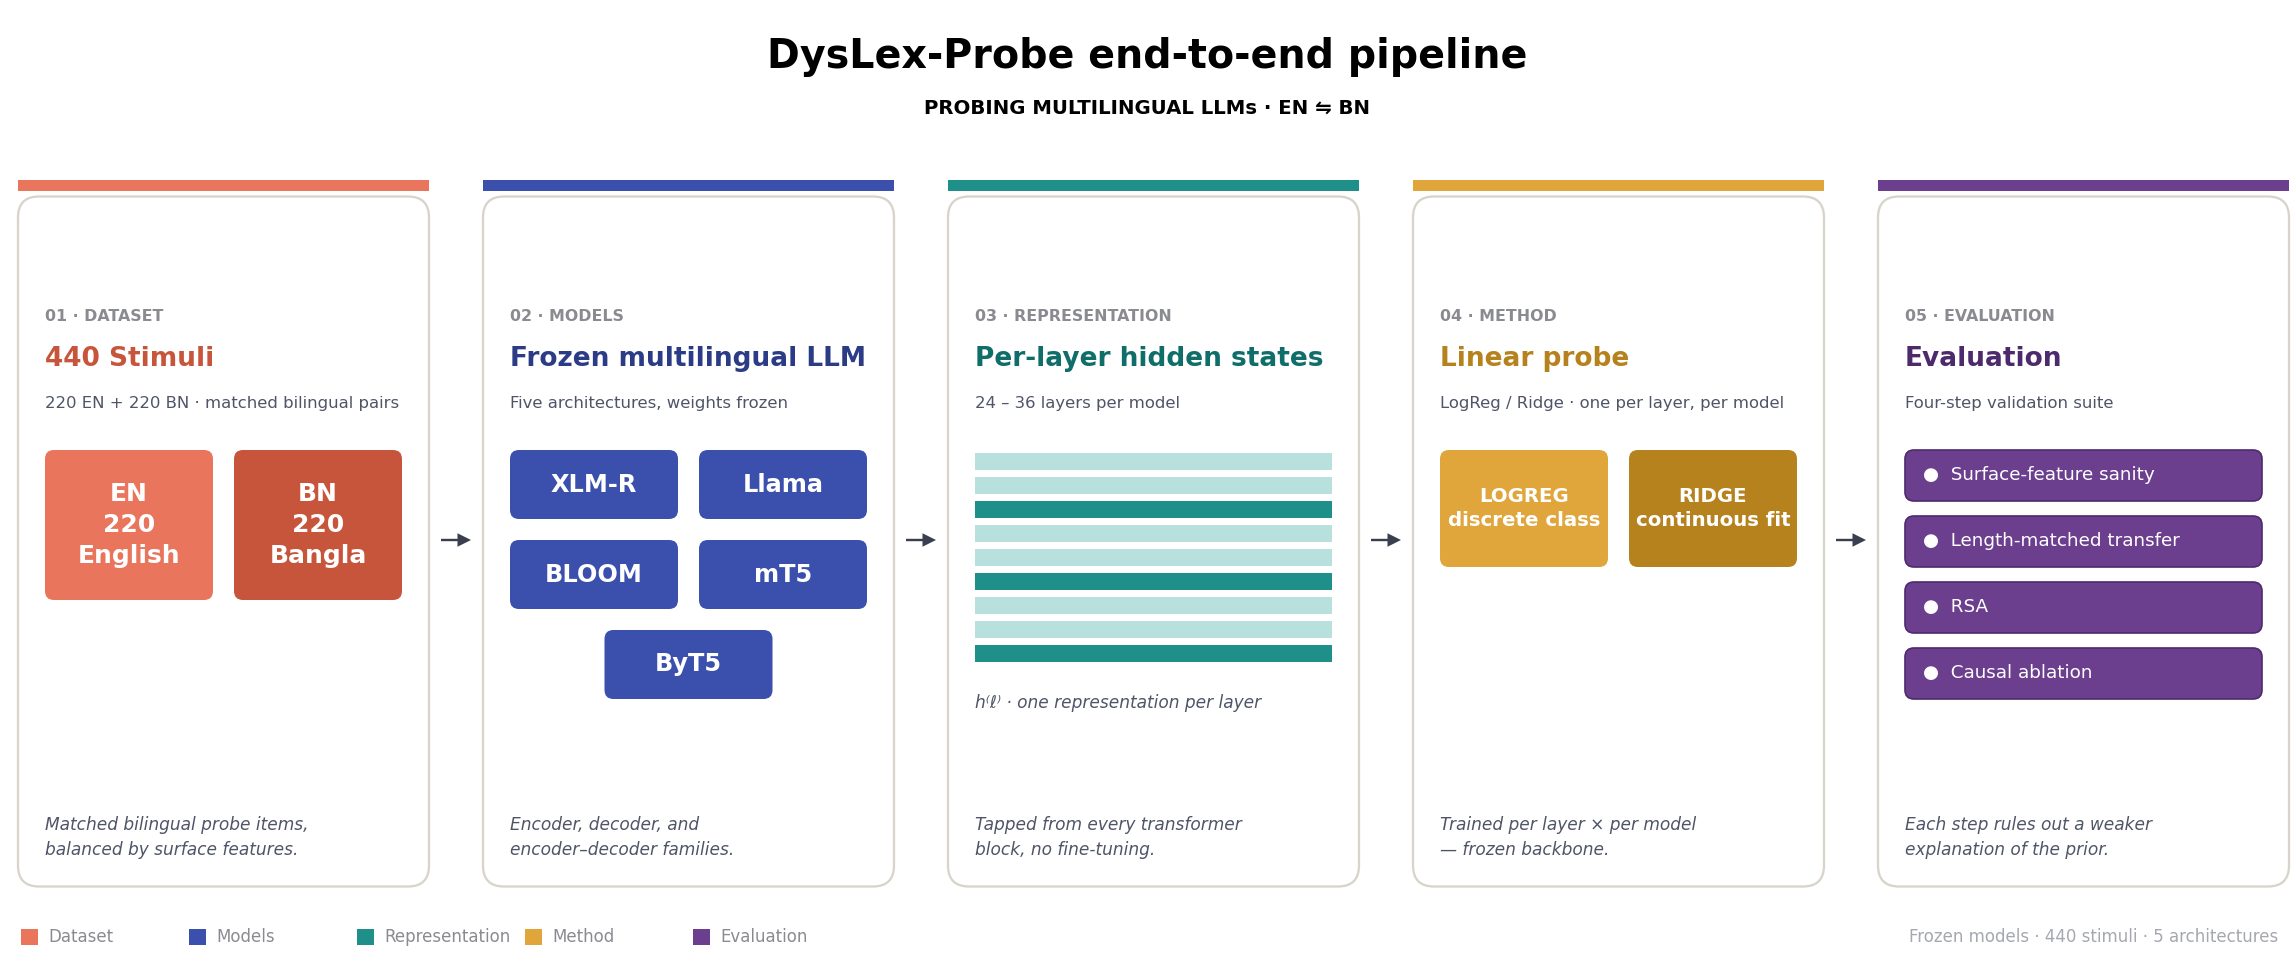
\includegraphics[width=0.92\linewidth]{fig_pipeline.png}
\caption{End-to-end probing pipeline. The 440-item English/Bangla dataset is fed through each frozen multilingual LLM; per-layer hidden states are extracted, a linear probe is trained on English, and representations are evaluated under surface-feature sanity checks, length-matched cross-lingual transfer, RSA and causal ablation, with bootstrap confidence intervals on all headline comparisons.}
\label{fig:pipeline}
\end{figure}

\subsection{Probing tasks and labels}
Four label sets are probed. \emph{Voicing} in binary, includes voiced and unvoiced. \emph{Real versus pseudoword} is binary, applied to the union of real word and pseudoword categories, and for surface controlling reporting, to the length matched subset. \emph{Orthographic transparency} is also binary which includes transparent and opaque categories. \emph{Syllable count} is an integer regression target. For every layer of every model, each task is probed and the per layer is selected by cross validation within the English training split.

\subsection{Surface feature sanity controls}
To ensure the validity of our claim, we performed surface feature sanity checks by implementing three strict control baseline. First, a first-character lookup baseline, which is a leave-one-out probe on the layer-0 token embedding. This quantifies how much of a label is recoverable from the first character alone. Second, a five feature character statistic baseline, the features are character length, byte length, unique character count and related surface counts. Any LLM probe that does not exceed this by more than 0.03 is not contributing to any information above surface statistics. Third, we enforced a strict 1:1 character length match between real and pseudo words. The evidence is measured by gain over surface, and not gain over chance.

\subsection{Representational Similarity Analysis}
We compute the cosine Representational Dissimilarity Matrix (RDM) \cite{kriegeskorte2008rsa} within each language and correlate the English and Bangla RDMs by Spearman $\rho$, it is performed on every layer. We also report English to Bangla mate retrieval Top-1 accuracy. Since RSA requires no probe training, and so it corroborates the probing result with an independent geometry only measure.

\subsection{Causal ablation and localization}
We quantify localization in two complementary ways on the surviving task. A \emph{causal forward hook ablation} brings the top-$K$ probe ranked hidden units at an earlier encoder block to zero and measures Bangla transfer downstream. It performs against a random unit control with multiple seeds, where \emph{specificity} is the ranked unit drop subtracted from the random unit drop. While this causal measure is applied to the four canonical models, the mT5 encoder is reablated at five depths to test for persistent ``backbone'' units. Because the residual stream is regenerating a forward hook intervention propagated through ByT5's much deeper, 36 layers, encoder before the measurement layer, we additionally used a propagation free \emph{direct} localization measure for the comparison of the five models including ByT5. We zero the top-20 probe ranked units of peak layers from each model in the representation itself and compare the Bangla drop against random unit zeroing. The both measures indicating localization agree for mT5, and direct measure avoids the depth confound while making it the fair basis for the comparison in between mT5 and ByT5.

\subsection{Bootstrap confidence intervals}
Every headline comparison is reported with a 95\% bootstrap confidence interval \cite{efron1994bootstrap} obtained by resampling the Bangla evaluation items with replacement (5000 resamples). For the both encoder-decoders and for the all five models we use a \emph{paired} bootstrap over the same resampled item indices. This yields confidence intervals on each model and on the between model differences (e.g.\ ByT5 minus mT5). A difference becomes significant when its interval excludes zero, and a transfer result ``survives'' when its interval lies entirely above the surface baseline.

\subsection{Downstream screening property classifier}
\label{sec:method-downstream}
In order to translate probing into an expert system relevant task, we train a classifier on English representations at the English selected layer and evaluate it zero shot on Bangla for each model and for a surface feature baseline. The targets are dyslexia relevant item properties present in the metadata. The real/pseudoword status such as lexical decision and the clinical marker, the targeted dyslexia error type, an 8-class label restricted to the error types present in both languages, item difficulty evaluated by ROC-AUC on hard versus not, and phonological complexity (three classes). Because the dataset comprises curated stimuli rather than clinical responses, this measures cross lingual transfer of item properties usable for screening item construction and grading, not patient level diagnosis. We report it with this scope stated explicitly and with the surface baseline as the reference every model must beat.

\subsection{Reproducibility}
Every reported number corresponds to a deterministic CSV in a per model results directory, with fixed seeds for probe training and multiple seeds for ablation random-unit controls. Probe uses L2-regularised logistic and ridge regression with fixed splits and majority class of classification and mean predictor of regression chance baselines. Pinned library and CUDA versions are recorded so the study is regenerable end to end on a single consumer GPU.

% ===========================================================================
\section{Results}
\label{sec:results}

\subsection{RQ1: most standard task fail sanity checks}
At very first sight In-language English probing recovers all four tasks (Table~\ref{tab:rq1}). But, the sanity checks reframe three of them. A layer-0 leave-one-out probe scores F1 0.78 to 0.94 across models (Fig.~\ref{fig:voicing}) essentially making Bangla voicing labels recoverable from the first character. So, the probe reads letter identity, not phonological voicing. Byte level ByT5 especially clarifies this by reaching its voicing peak at the very first layer (L1, F1 0.97) (Fig.~\ref{fig:byt5profile}a). It is possible because at the byte level the first character is directly available at the embedding. Orthographic transparency is solved by using the five feature surface baseline (EN F1 0.66, BN 0.82), with the LLMs adding at most $+0.03$. Syllable count is surface-confounded (EN surface $R^2$ 0.81), and most models fall to or below the surface baseline while only real versus pseudoword survives.

\begin{table}[H]
\caption{RQ1 in-language English probing: peak layer / peak score per model per task (F1; $R^2$ for syllable). Daggered tasks fail surface-feature sanity checks. ByT5's early voicing peak (L1) reflects direct byte-level access to the first character.}
\label{tab:rq1}
\centering
\small
\setlength{\tabcolsep}{4pt}
\begin{tabular}{lccccc}
\toprule
\textbf{Task} & \textbf{XLM-R} & \textbf{Llama} & \textbf{BLOOM} & \textbf{mT5} & \textbf{ByT5} \\
\midrule
Voicing$^\dagger$    & L11/0.62 & L2/0.73  & L6/0.55  & L9/0.58  & L1/0.97 \\
Realword             & L11/0.84 & L12/0.91 & L22/0.79 & L24/0.81 & L23/0.72 \\
Ortho$^\dagger$      & L0/0.92  & L32/0.71 & L12/0.68 & L21/0.69 & L9/0.72 \\
Syllable$^\dagger$   & L8/0.67  & L16/0.70 & L29/0.68 & L20/0.76 & L28/0.90 \\
\bottomrule
\end{tabular}
\end{table}

\begin{figure}[tbp]
\centering
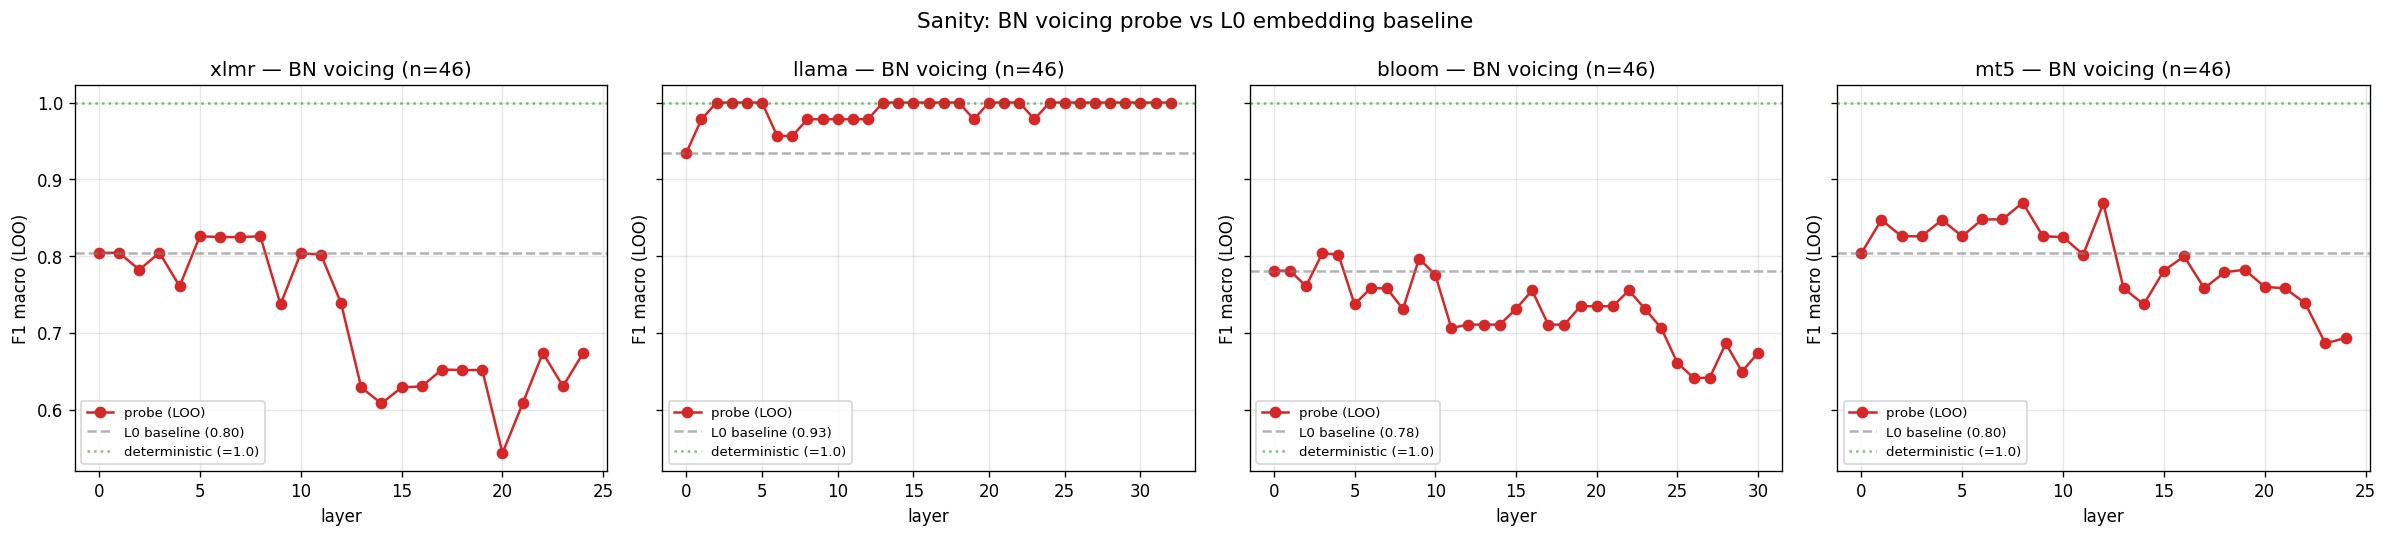
\includegraphics[width=0.9\linewidth]{plots_bn_voicing_sanity.png}
\caption{Bangla voicing sanity check on the four canonical (subword/BPE) models: a leave-one-out probe on layer-0 token embeddings recovers the voicing label at F1 0.78--0.94, demonstrating that the label is inferable from first-character identity alone rather than from phonological voicing. Byte-level ByT5 shows the same confound even more directly, peaking at its first layer (F1 0.97), and is plotted separately in Fig.~\ref{fig:byt5profile}a.}
\label{fig:voicing}
\end{figure}

\subsection{Length matched recovery}
When real and pseudo words are matched 1:1 on character length, all five models exceed both their layer-0 and the surface baseline on Bangla (Table~\ref{tab:realword}). This is the only task that passes the surface controls, RSA and ablation numbers. It is the basis for all subsequent transfers. Despite having a weaker in-language English peak of 0.80, ByT5 gains $+0.27$ on Bangla, which gives the first hint that byte level tokenization trades some monolingual precision for stronger cross lingual sharing.

\begin{table}[H]
\caption{Length-matched realword probing per language: layer-0 vs peak F1, with gain over layer~0. All five models gain substantially on Bangla.}
\label{tab:realword}
\centering
\small
\setlength{\tabcolsep}{4pt}
\begin{tabular}{lcccccc}
\toprule
& \multicolumn{3}{c}{\textbf{English}} & \multicolumn{3}{c}{\textbf{Bangla}} \\
\cmidrule(lr){2-4}\cmidrule(lr){5-7}
\textbf{Model} & L0 & peak & gain & L0 & peak & gain \\
\midrule
XLM-R & 0.81 & 0.88 & $+0.06$ & 0.66 & 0.92 & $+0.25$ \\
Llama & 0.75 & 0.96 & $+0.21$ & 0.64 & 0.90 & $+0.26$ \\
BLOOM & 0.81 & 0.94 & $+0.13$ & 0.64 & 0.94 & $+0.30$ \\
mT5   & 0.65 & 0.90 & $+0.23$ & 0.72 & 0.92 & $+0.20$ \\
ByT5  & 0.57 & 0.80 & $+0.13$ & 0.65 & 0.92 & $+0.27$ \\
\bottomrule
\end{tabular}
\end{table}

\subsection{RQ2: cross lingual transfer splits the models, with confidence intervals}
The English trained length matched probe clearly separates the models (Table~\ref{tab:results}) (Fig.~\ref{fig:forest}) when evaluating zero shot on Bangla. BLOOM and ByT5 both achieved genuine transfer with 0.92 F1, 95\% CI [0.84, 0.98] and XLM-R (0.86, [0.75, 0.94]) also achieved genuine transfer. Their intervals lie entirely above the surface baseline of 0.62, where Llama (0.63, [0.48, 0.77]) and mT5 (0.60, [0.45, 0.74]) collapse as their intervals straddle the surface. Three implications follow from this. First, pretraining coverage and objective \emph{jointly} determine transfer. BLOOM with explicit Bangla coverage beats Llama at a similar scale. The 0.56B XLM-R also beats the 8B Llama while having roughly 13$\times$ fewer parameters. Second, in language English performance is unpredictable, but Llama has the highest English realword F1 at 0.96 and the lowest Bangla transfer with 0.63 F1. Third, the negative gain of mT5 ($-0.02$) is not anti-learning. It means the representation scores marginally below the surface baseline, i.e.\ zero transfer within the $n = 50$ estimation noise. The forest plot (Fig.~\ref{fig:forest}, left) shows the intervals directly.

\begin{table}[H]
\caption{Headline surface-controlled results with 95\% bootstrap confidence intervals. Zero-shot cross-lingual real-versus-pseudoword F1 on the length-matched subset ($n{=}50$ per language), gain over the surface baseline (0.62), the paired direct-ablation localization specificity, and the resulting verdict.}
\label{tab:results}
\centering
\small
\setlength{\tabcolsep}{3pt}
\begin{tabular}{lcccl}
\toprule
\textbf{Model} & \textbf{Transfer BN F1 [95\% CI]} & \textbf{Gain} & \textbf{Spec.\ [95\% CI]} & \textbf{Verdict} \\
\midrule
XLM-R  & 0.86 [0.75, 0.94] & $+0.24$ & $+0.14$ [0.05, 0.24] & survive, local. \\
BLOOM  & \textbf{0.92} [0.84, 0.98] & $+0.30$ & $+0.00$ [0.00, 0.00] & survive, distrib. \\
ByT5   & \textbf{0.92} [0.84, 0.98] & $+0.30$ & $+0.01$ [0.00, 0.04] & survive, distrib. \\
Llama  & 0.63 [0.48, 0.77] & $+0.01$ & $-0.06$ [-0.12, -0.01] & collapse \\
mT5    & 0.60 [0.45, 0.74] & $-0.02$ & $+0.19$ [0.06, 0.32] & collapse, local. \\
\bottomrule
\end{tabular}
\end{table}

\begin{figure}[tbp]
\centering
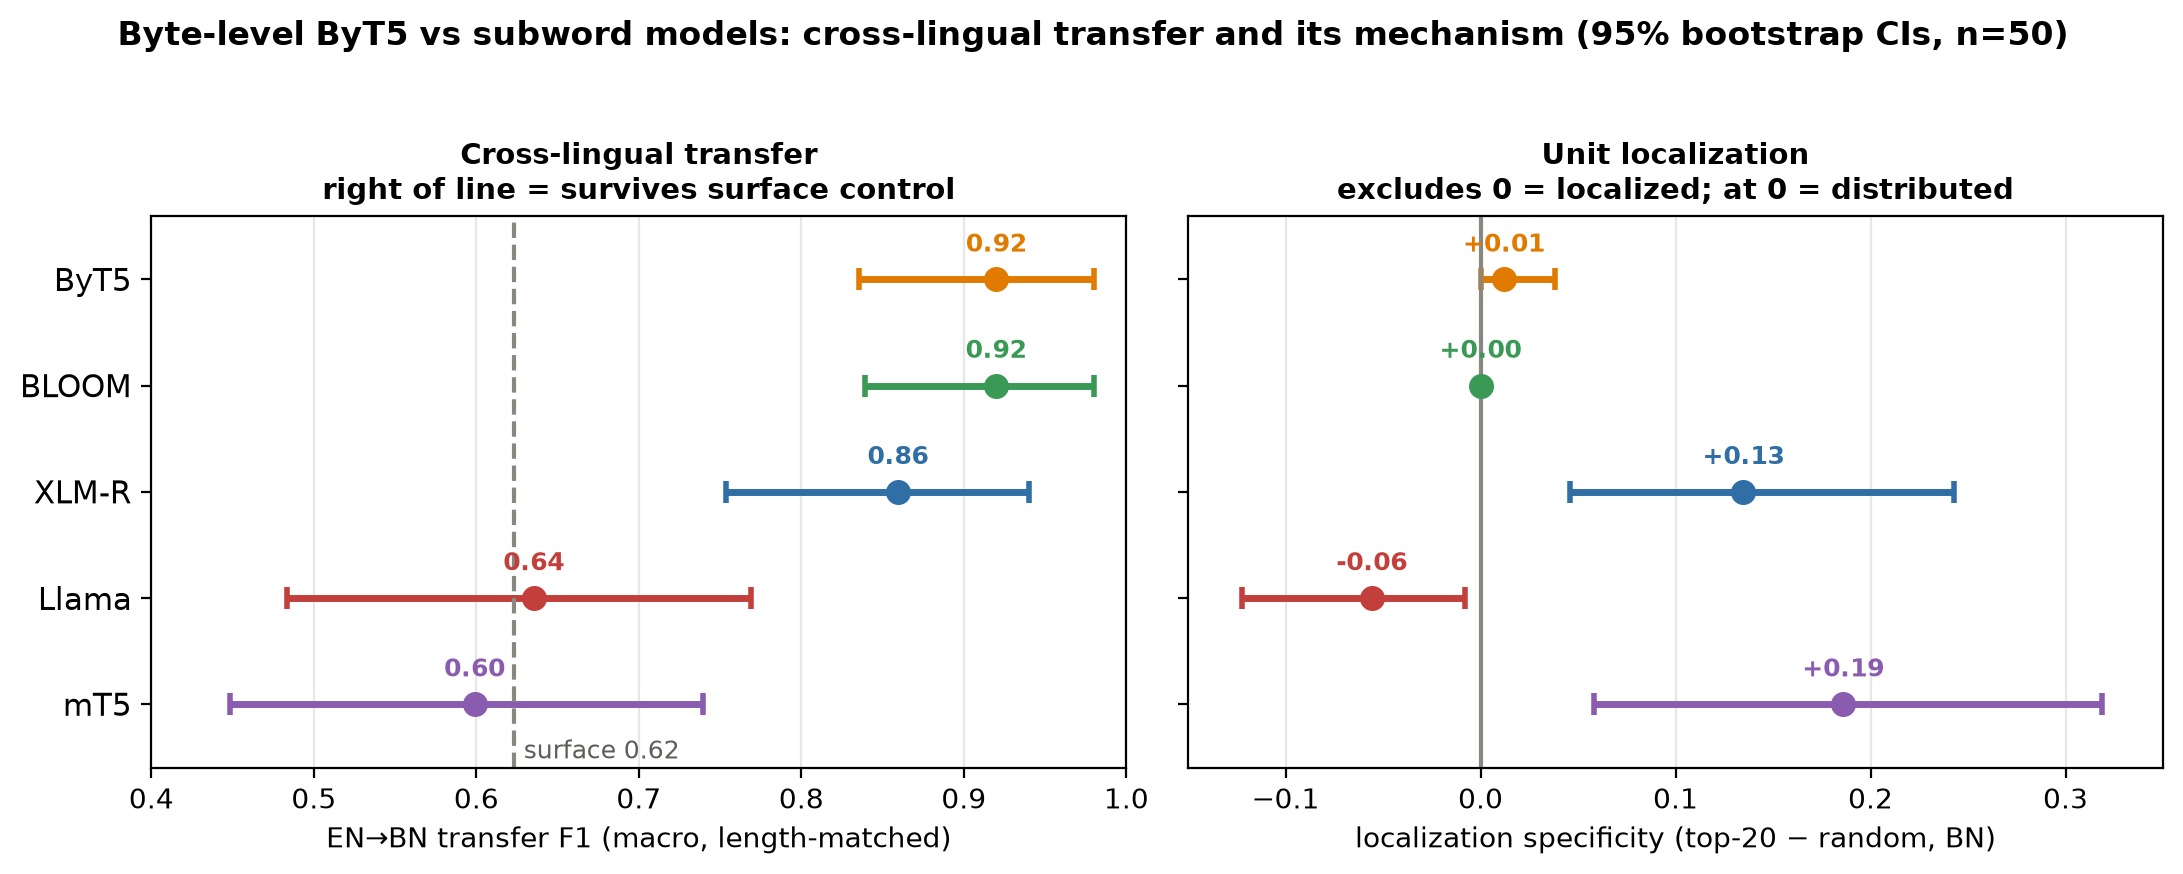
\includegraphics[width=0.99\linewidth]{plots_bootstrap_ci_forest.png}
\caption{Bootstrap 95\% confidence intervals for all five models. Left: cross-lingual transfer F1 against the surface baseline (dashed); intervals right of the line survive the surface control (XLM-R, BLOOM, ByT5). Right: direct-ablation localization specificity against zero; intervals excluding zero indicate a localized signal (mT5, XLM-R), while intervals at zero indicate a distributed signal (BLOOM, ByT5).}
\label{fig:forest}
\end{figure}

\subsection{RQ3: tokenization is decisive -- ByT5 versus mT5}
\label{sec:tokenization}
Although both the encoder-decoder models from a controlled pair share architecture and span corruption pretraining, they mainly differ in tokenization. The contrast is sharply clear (Fig.~\ref{fig:byt5}). mT5 with subword tokens collapse having F1 0.60, while ByT5 with byte-level tokenization is best in class with F1 0.92. The paired difference of them is $+0.32$ (95\% CI [0.15, 0.49]) which is well clear of zero. Since the objective and architecture are held fixed, \emph{tokenization} can be identified as the cause of mT5's cross lingual collapse. This corrects the intuition that the collapse reflects the span corruption encoder-decoder objective. The most probable mechanism is representational. On one hand, a byte-level model places English and Bangla in a single shared 256-symbol input space by aligning cross lingual lexical structure. On the other hand, a subword vocabulary trained largely on Latin script gives the two scripts nearly disjoint token inventories. Consistent with this, ByT5's advantage appears across the encoder depth (Fig.~\ref{fig:byt5}) over mT5 rather than at a single layer, and it is accompanied by a slightly weaker monolingual English peak (Table~\ref{tab:realword}), exactly the trade off a shared space account predicts.

The behaviour of the byte encoder became concrete due to its internal profile (Fig.~\ref{fig:byt5profile}): in language, voicing peaks at the first layer as it gets direct byte access to the initial character. But, real versus pseudoword and orthographic structure build gradually through the deep encoder, and the length matched cross lingual probe climbs from chance to its 0.92 Bangla peak at layer 29 by crossing the surface baseline midway up the 36-layer stack. We noted one honest caveat: ByT5 also has a deeper encoder, so the cleanest statement is that byte level ByT5, unlike subword mT5, transfers, with tokenization the most probable single driver.

\begin{figure}[tbp]
\centering
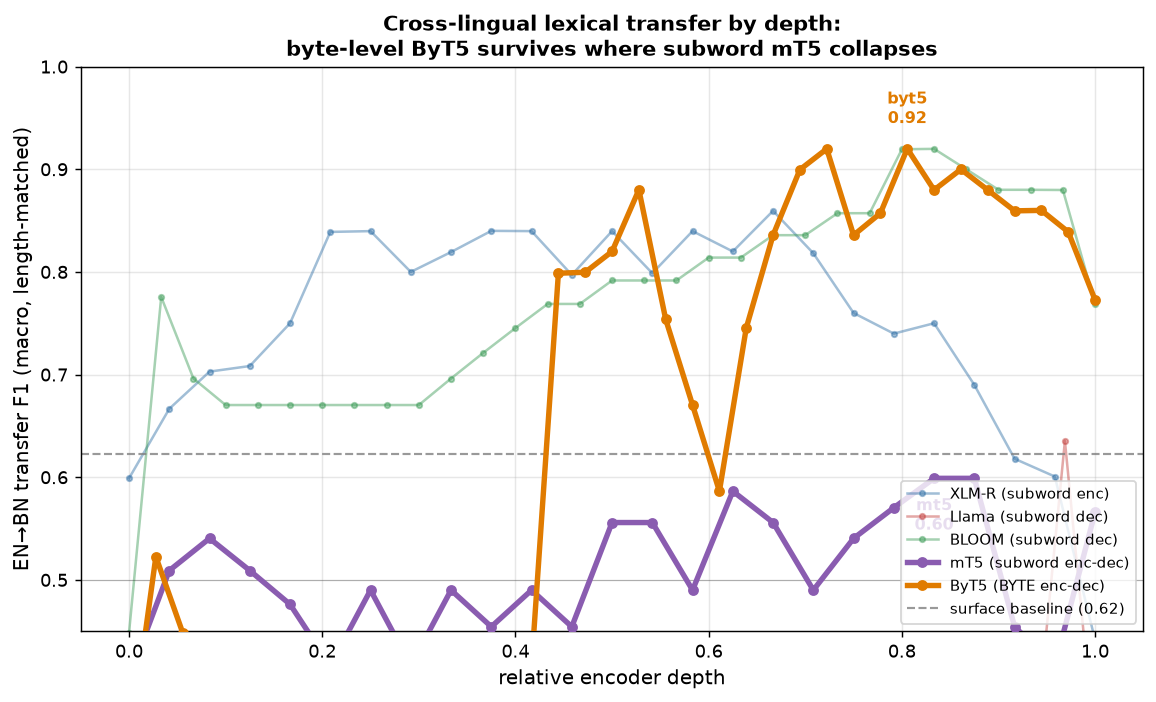
\includegraphics[width=0.99\linewidth]{plots_byt5_vs_mt5_transfer_emergence.png}
\caption{Per-layer cross-lingual transfer against relative encoder depth. Byte-level ByT5 (emphasised) rises to 0.92 F1 while subword mT5 (emphasised) hugs the surface baseline; the two share architecture and pretraining objective and differ chiefly in tokenization. The other three models are shown faded for context.}
\label{fig:byt5}
\end{figure}

\begin{figure}[tbp]
\centering
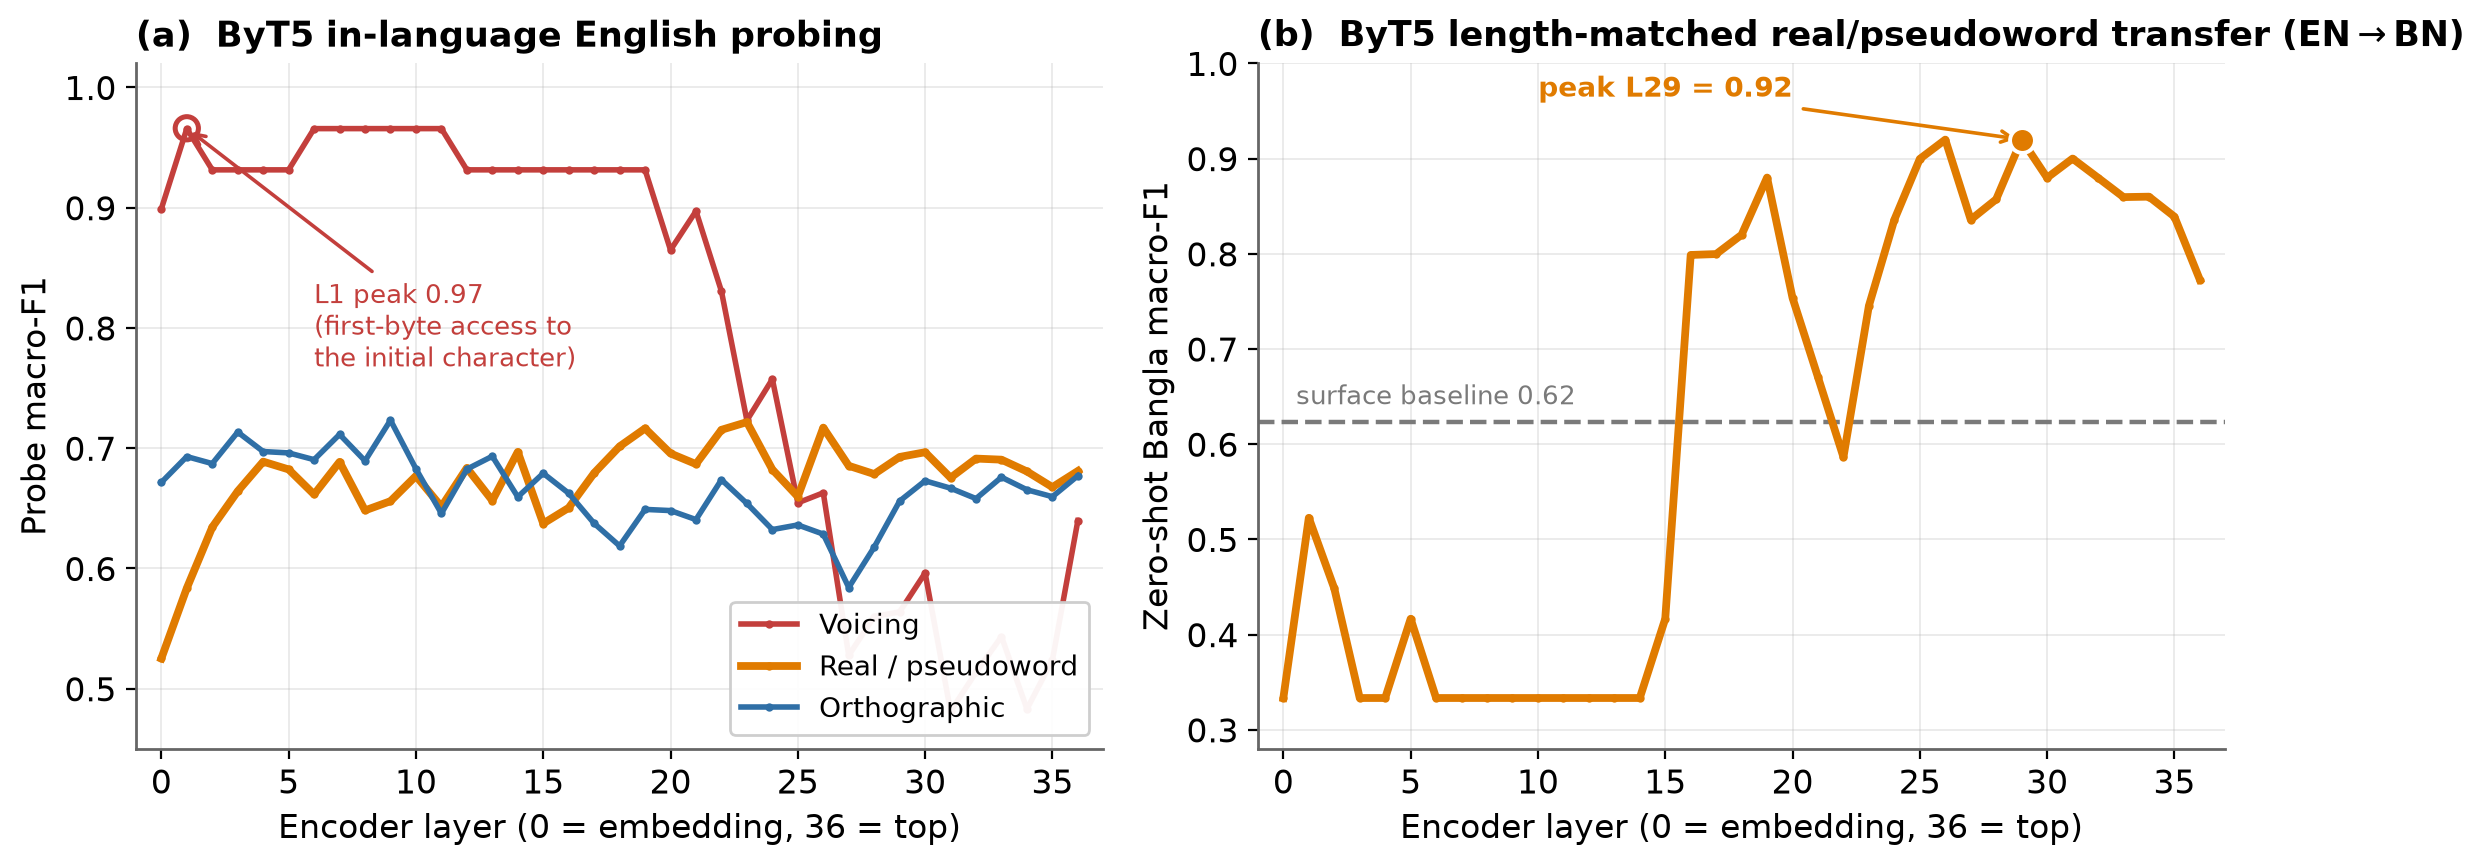
\includegraphics[width=0.99\linewidth]{plots_byt5_probing_profile.png}
\caption{ByT5 byte-level probing profile. (a)~In-language English per-layer probe scores: voicing peaks at layer~1, because at the byte level the first character is directly available at the embedding, whereas real-versus-pseudoword and orthographic structure emerge deeper in the 36-layer encoder. (b)~The length-matched real-versus-pseudoword probe, trained on English and evaluated zero-shot on Bangla, rises from chance to 0.92 F1 at layer~29, crossing the surface baseline (dashed) midway up the encoder. The regression syllable-count target is omitted from~(a) for scale.}
\label{fig:byt5profile}
\end{figure}

\subsection{RSA corroborates the transfer split}
RSA agrees with the probing result. Cross lingual RDM Spearman $\rho$ and English to Bangla mate retrieval Top-1 peak at mid layers for the transferring sub word models. XLM-R reaches its highest cross lingual RDM correlation in its middle encoder layers, coincidently, with the layer at which the length matched real word probe transfers. Llama reaches a high Top-1 in the \emph{unmatched} RSA setting, but this is driven by the same surface confound that inflates its unmatched probing numbers and disappears under matching. The informative exception is byte level ByT5 (Table~\ref{tab:rsa}). It transfers strongly on the supervised lexical probe yet shows only modest concept match RSA, peak $\rho$ 0.21 at L29 (Top-1 0.25), because its byte level code aligns cross lingual lexical \emph{form} rather than cross script \emph{semantics} that the concept match pairs probe. With byte sequences disjoint across the two scripts this residual alignment cannot be a surface artefact, so it is genuine but partial. Representational geometry is therefore preserved cross-lingually in the subword transferring models, only weakly in the byte-level model, and not in mT5.

\begin{table}[H]
\caption{RSA summary: peak cross-lingual RDM Spearman $\rho$ and English$\to$Bangla mate-retrieval Top-1, with whether the signal survives length matching.}
\label{tab:rsa}
\centering
\small
\setlength{\tabcolsep}{5pt}
\begin{tabular}{lccc}
\toprule
\textbf{Model} & \textbf{Peak RDM $\rho$} & \textbf{Peak Top-1} & \textbf{Survives matching} \\
\midrule
XLM-R & mid-encoder & high & yes \\
BLOOM & mid layers  & 0.65 & yes \\
ByT5  & 0.21 (L29)  & 0.25 & partial (form-based) \\
Llama & --          & 0.85$^\ast$ & no (surface) \\
mT5   & 0.244 (L15) & low  & no \\
\bottomrule
\end{tabular}
\\[2pt]
{\footnotesize $^\ast$Unmatched setting; driven by surface confound, vanishes under matching.}
\end{table}

\subsection{RQ4: localization and a double dissociation}
Causal ablation distinguishes how the signal is stored. Under the causal forward-hook measure on the four canonical models (Fig.~\ref{fig:ablation}), only mT5 shows clean specificity: zeroing its top-ranked encoder units selectively impairs Bangla transfer (specificity $+0.11$), whereas XLM-R and BLOOM are distributed and Llama has no transfer to disrupt. Repeating the ablation across five mT5 encoder depths (Table~\ref{tab:depth}) the effect persists at every depth and peaks in the mid encoder (L12, $+0.13$). While most units are layer specific, unit 782 and unit 1880 recur in the top ranked set across depths and form a persistent backbone (Fig.~\ref{fig:backbone}). A hybrid of a small persistent backbone plus layer-local specialised circuits.

Extending the analysis to all five models with the propagation-free direct measure and bootstrap intervals reveals a clean \emph{double dissociation} (Table~\ref{tab:results}, Fig.~\ref{fig:forest} right). The localized models are mT5 ($+0.19$, 95\% CI [0.06, 0.32]) and XLM-R ($+0.14$, [0.05, 0.24]), both subword and both with an encoder, while BLOOM ($0.00$) and byte-level ByT5 ($+0.01$, [0.00, 0.04]) distribute the signal. Llama's negative value is not interpretable as it has no transfer to localize. Crucially, the tokenization flips the mechanism among the controlled encoder-decoder pair. The paired mT5 and ByT5 specificity difference is $+0.17$ (95\% CI [0.05, 0.31]), which is significant. Byte-level tokenization thus changes not only whether cross-lingual lexical structure transfers but how it is organised. The byte-level, shared-space code is distributed and robust, the subword code sparse and localized. (The direct measure gives mT5 $+0.19$ where the forward-hook measure gives $+0.11$; the two methods agree on the qualitative conclusion that mT5 localizes, and we use the direct measure only where a fair ByT5 comparison is required.)

\begin{figure}[tbp]
\centering
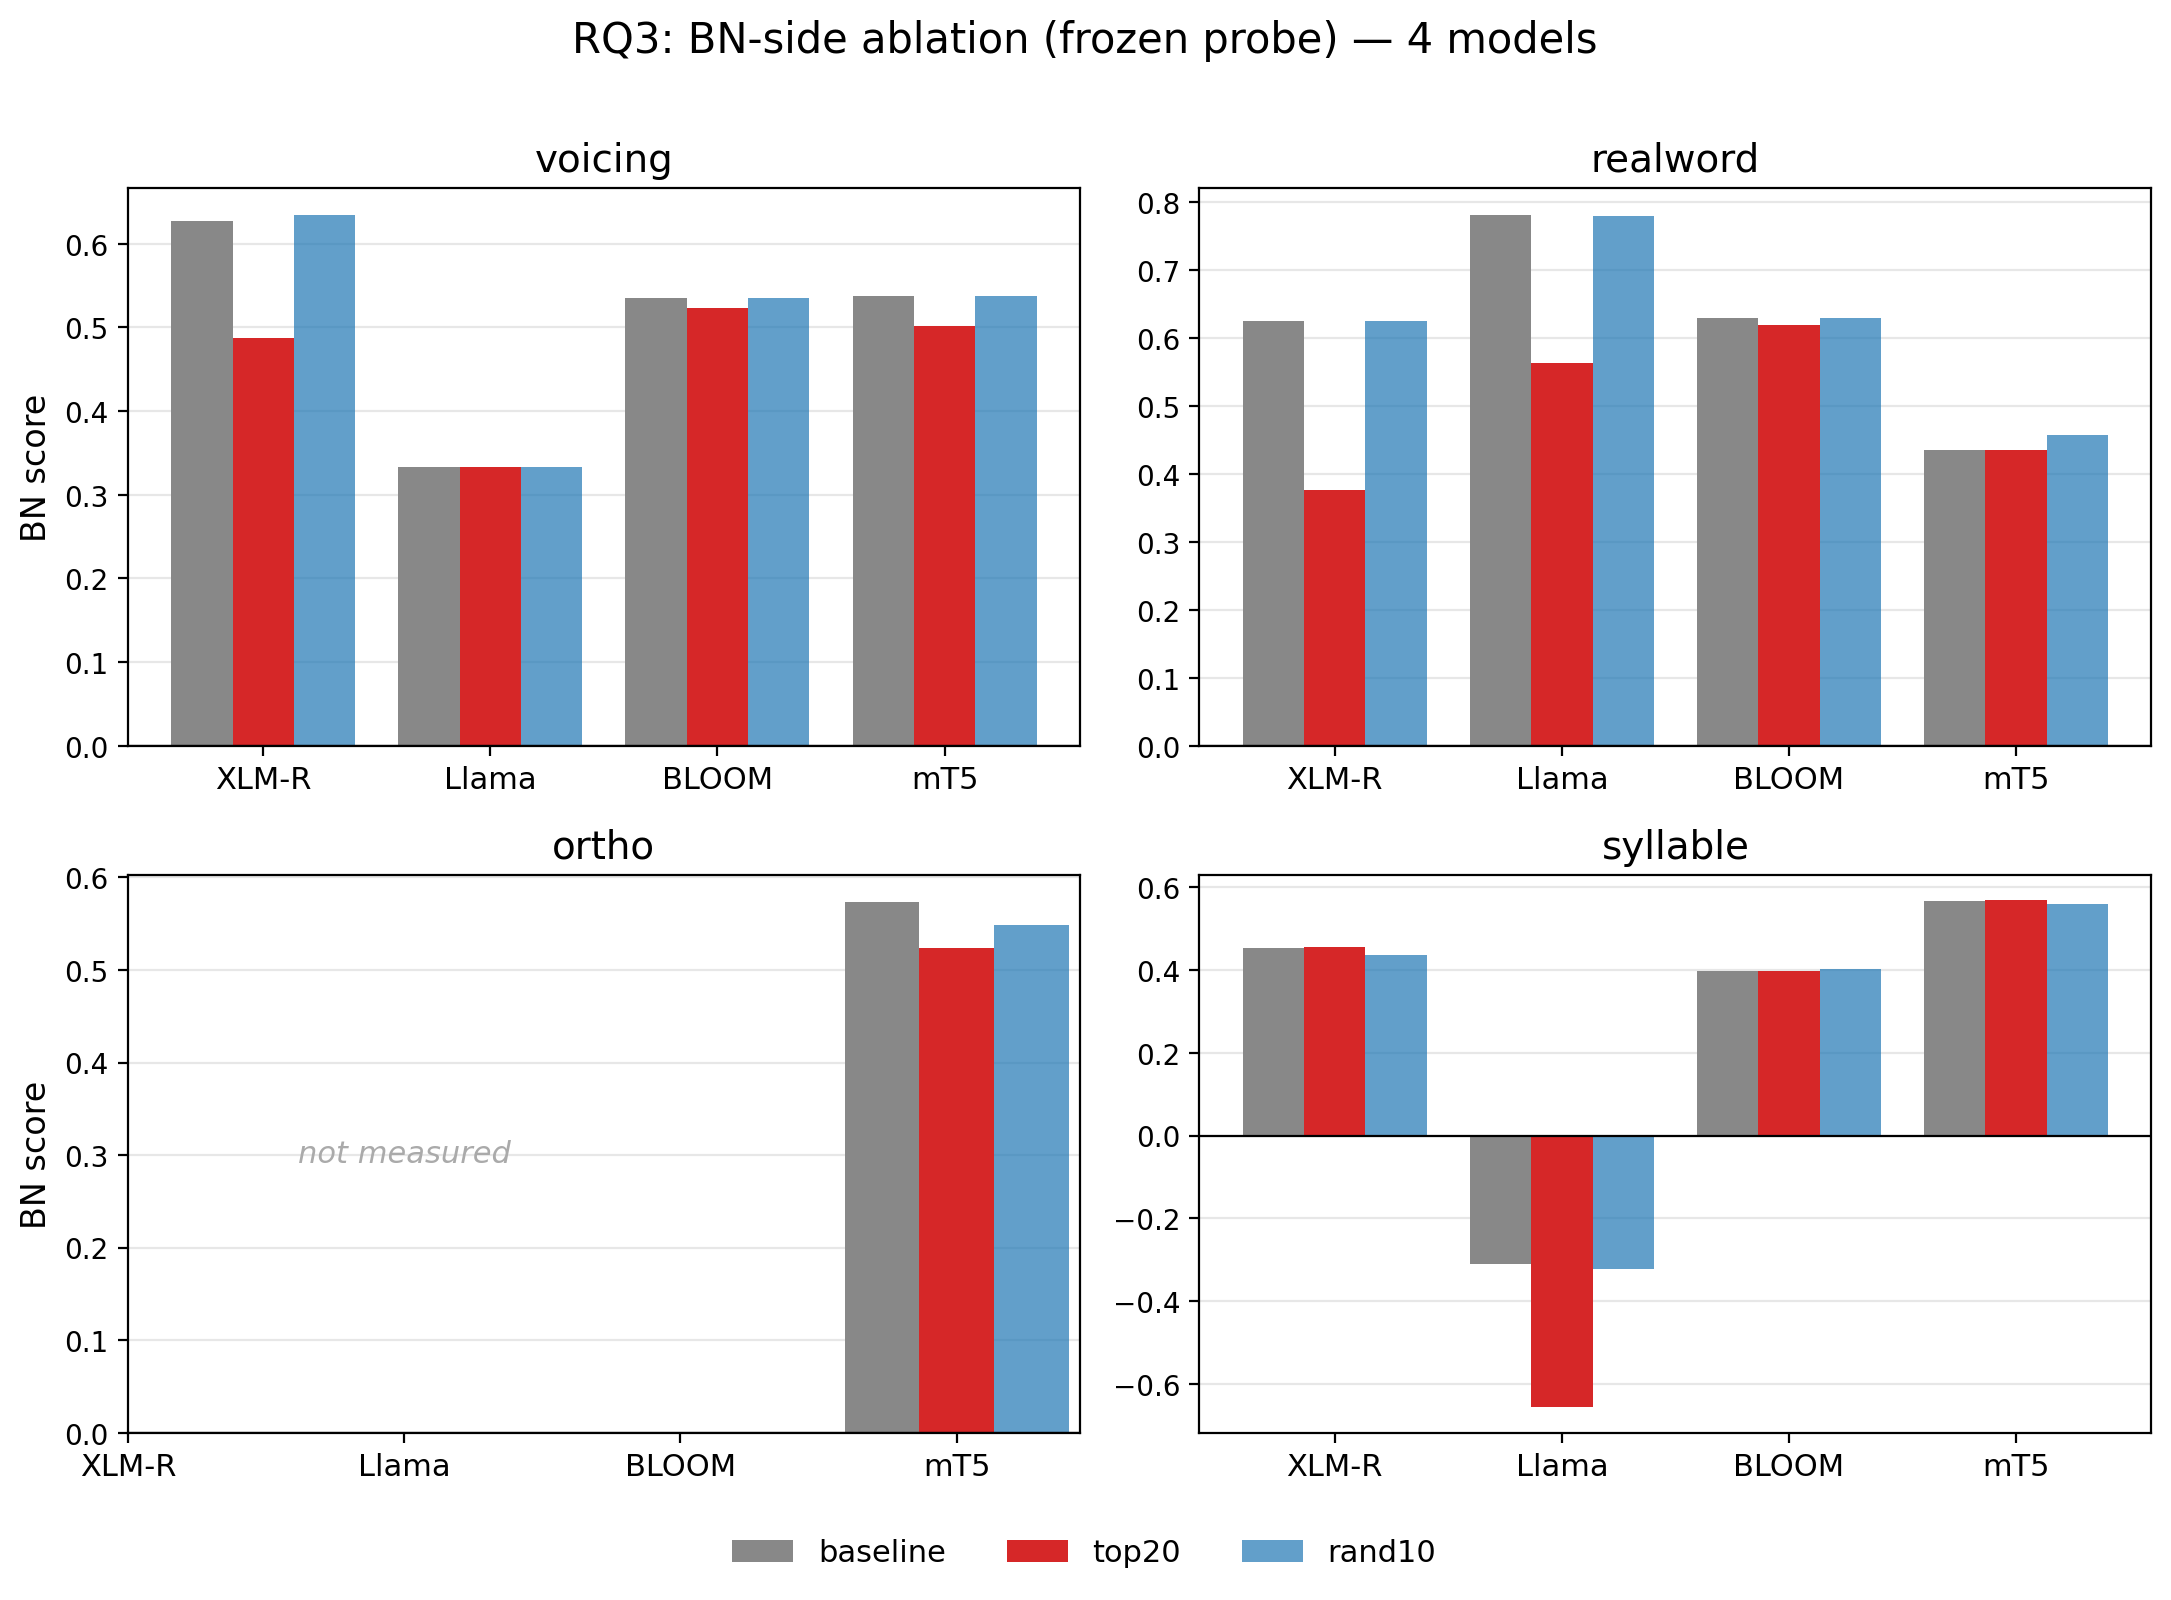
\includegraphics[width=\linewidth]{plots_four_models_ablation_2x2.png}
\caption{Four-model causal forward-hook ablation across the four probing tasks: top-20 versus random-10 unit ablation on the Bangla cross-lingual probe; ortho was measured for mT5 only. Only mT5 shows clean specificity; XLM-R, BLOOM and Llama do not. ByT5 is assessed with the propagation-free direct measure instead (Fig.~\ref{fig:forest}, right; Table~\ref{tab:results}), because a forward-hook signal is regenerated before the measurement layer in its deeper 36-layer encoder.}
\label{fig:ablation}
\end{figure}

\begin{table}[H]
\caption{mT5 encoder forward-hook ablation across depth: top-10 vs random-mean specificity per measurement layer (three seeds). Localization persists across depth; mid-encoder (L12) is strongest.}
\label{tab:depth}
\centering
\small
\setlength{\tabcolsep}{5pt}
\begin{tabular}{lcccc}
\toprule
\textbf{Depth} & \textbf{BN base} & \textbf{Top-10 drop} & \textbf{Rand mean} & \textbf{Specificity} \\
\midrule
L4  & 0.48 & $+0.06$ & $0.00$ & $+0.06$ \\
L8  & 0.49 & $+0.07$ & $0.00$ & $+0.07$ \\
\textbf{L12} & 0.56 & \textbf{$+0.14$} & $0.01$ & \textbf{$+0.13$} \\
L16 & 0.56 & $+0.03$ & $-0.01$ & $+0.04$ \\
L20 & 0.60 & $+0.11$ & $0.00$ & $+0.11$ \\
\bottomrule
\end{tabular}
\end{table}

\begin{figure}[tbp]
\centering
\makebox[\linewidth][c]{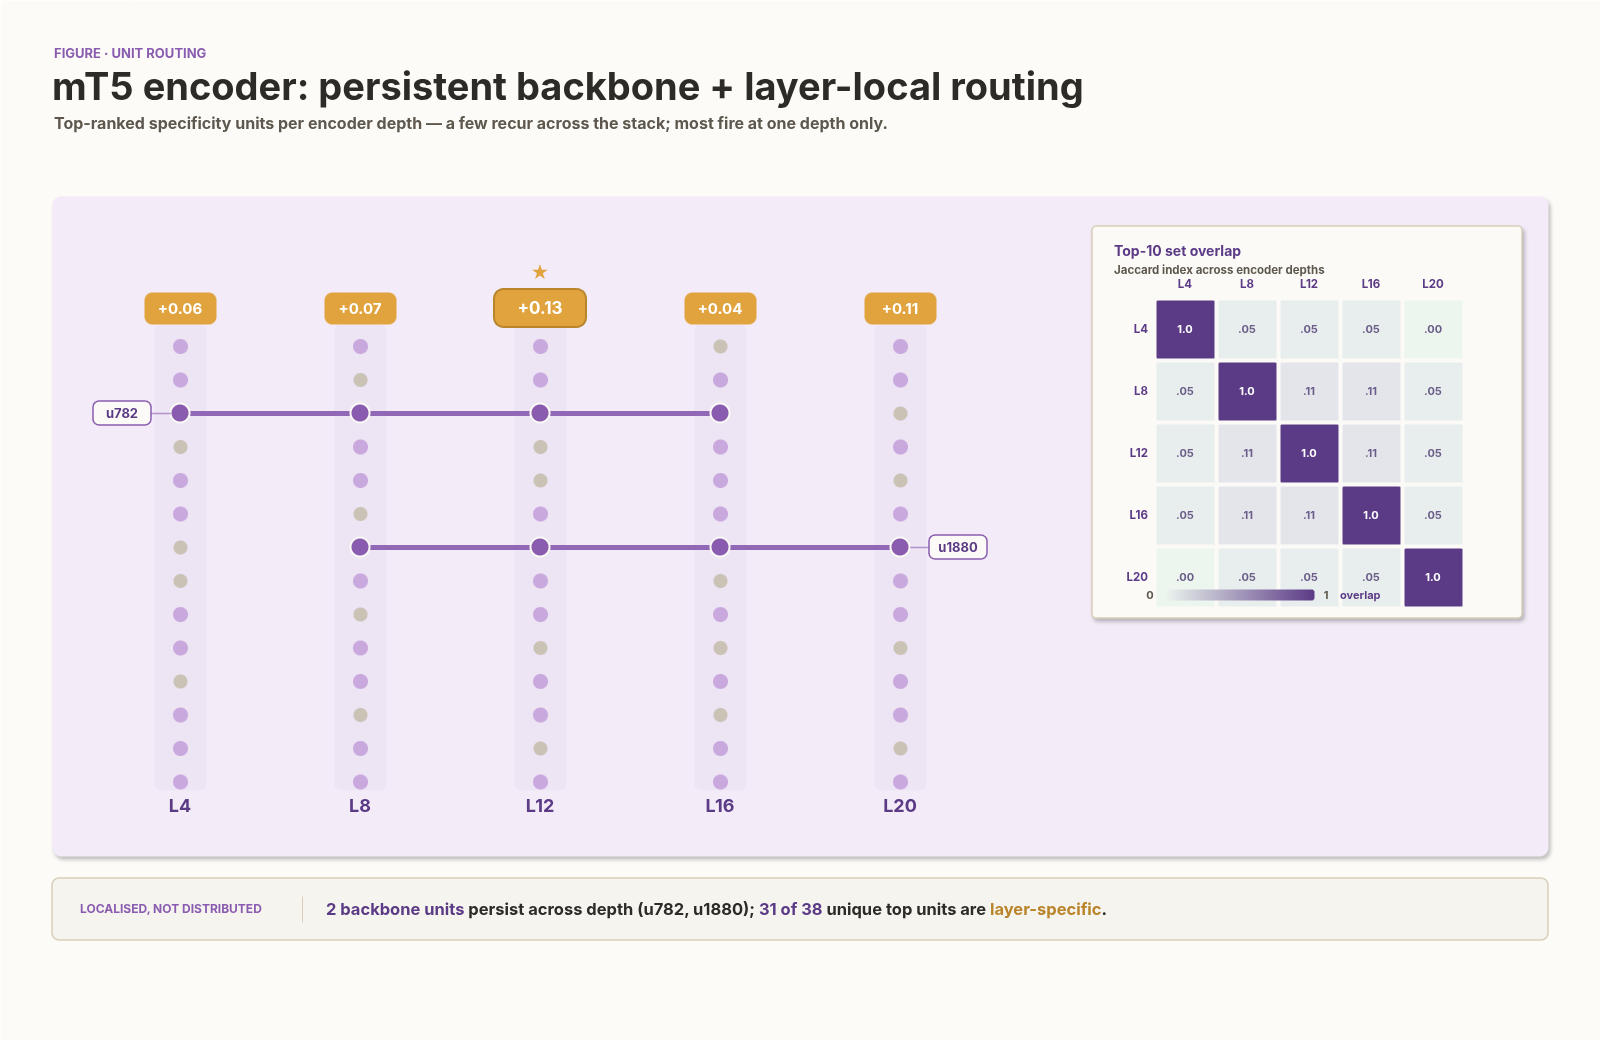
\includegraphics[width=1.35\linewidth]{fig_mt5_backbone.png}}
\caption{mT5 encoder localization across depth. Two backbone units (u782, u1880) recur in the top-ranked set across most probed depths, while the remaining top units are layer-specific; per-depth ablation specificity peaks at L12. Inset: Jaccard overlap of the top-10 unit sets across depths.}
\label{fig:backbone}
\end{figure}

\subsection{RQ5: downstream screening property transfer}
\label{sec:downstream}

\begin{table}[H]
\caption{Downstream cross-lingual screening-property transfer (train English, test Bangla): metric per model against the surface baseline. Lexical decision and error type are macro-F1; difficulty is ROC-AUC; complexity is macro-F1. Bold entries significantly beat the surface baseline (paired bootstrap CI excludes it).}
\label{tab:downstream}
\centering
\small
\setlength{\tabcolsep}{4.5pt}
\begin{tabular}{lcccccc}
\toprule
\textbf{Task (metric)} & \textbf{Surf.} & \textbf{XLM-R} & \textbf{Llama} & \textbf{BLOOM} & \textbf{mT5} & \textbf{ByT5} \\
\midrule
Lexical decision (F1)   & 0.62 & \textbf{0.86} & 0.64 & \textbf{0.92} & 0.60 & \textbf{0.92} \\
Error type (F1)         & 0.26 & 0.31 & 0.03 & 0.26 & 0.29 & \textbf{0.32} \\
Difficulty (AUC)        & 0.80 & 0.76 & 0.54 & 0.77 & 0.88 & 0.80 \\
Phon.\ complexity (F1)  & 0.37 & 0.31 & 0.28 & 0.33 & \textbf{0.48} & 0.23 \\
\bottomrule
\end{tabular}
\end{table}

Moving from probing to an expert-system-relevant task, we ask whether a classifier trained only on English item properties can grade Bangla items above a surface baseline (Table~\ref{tab:downstream}). The answer is a clean boundary. For categorical and lexical properties the LLMs add real signal. On lexical decision, real versus pseudo word, ByT5, BLOOM and XLM-R beat surface by $+0.24$ to $+0.30$, and on the 8-class dyslexia error type byte level ByT5 is the only model that significantly exceed the surface baseline with macro-F1 score at 0.322, paired $\Delta{=}{+}0.064$, 95\% CI (0.00, 0.13). For abstract, graded properties the LLMs do not help. On item difficulty (hard vs rest) no model significantly beats a strong surface baseline (ROC-AUC 0.795; mT5 highest at 0.878 but non-significant), and on three-class phonological complexity only mT5 marginally exceeds surface ($+0.10$, 95\% CI [0.00, 0.20]) while byte-level ByT5 falls significantly below it. The transferable, supra-surface signal is thus concentrated in categorical lexical distinctions, and is strongest under byte-level tokenization, the same property that drives the RQ2 transfer result. This bounds the honest scope of an LLM-based Bangla screening tool. It can help select and grade the lexical-decision items that matter clinically, but it does not replace surface heuristics for graded difficulty.

\subsection{Model selection}
No single model dominates every criterion. BLOOM and ByT5 are the best practical substrates for a Bangla lexical-screening prototype with highest transfer and 0.92 F1. XLM-R is the most parameter-efficient (0.86 F1 at roughly 13$\times$ fewer parameters). mT5 is the most interpretable (a recoverable, localized mechanism). Llama, despite being the largest, is not recommended for Bangla because its cross lingual transfer collapses. For a deployment that must run on modest hardware, XLM-R is the pragmatic default. Where interpretability of the screening signal is required, mT5. Where raw cross-lingual accuracy matters most and the tokenizer confound must be excluded, ByT5.

% ===========================================================================
\section{Economic and deployment feasibility}
\label{sec:cost}
One of the practical advantage of frozen probing is the cost. The full pipeline (five models $\times$ 440 stimuli $\times$ per-layer extraction, probing, RSA and ablation) of the model runs in a few tens of GPU-hours, using a single consumer GPU. Training a comparable Bangla-only model from scratch takes $10^{4}$ GPU-hours and a large labelled Bangla corpus that doesn't exist, but the frozen prototype path is roughly three orders of magnitude cheaper on direct compute and qualitatively infinite on data. For a clinical pilot study, a 4-bit quantized decoder or a 16-bit encoder can infer stimuli at an interactive pace. Even with 50 items per child and a testing volume of 1,000 children annually, the power consumption is negligible compared to the clinician's working time. This is the economic rationale particularly in resource constrained clinical NLP environments: before undertaking the costly process of fine tuning a model, it is more logical to adopt the surface-controlled frozen probing method on the same multilingual substrate as the default approach.

\begin{table}[H]
\caption{Approximate compute cost of the full pipeline on a single consumer GPU (electricity at BDT 11.5/kWh, 350~W average draw).}
\label{tab:cost}
\centering
\small
\setlength{\tabcolsep}{5pt}
\begin{tabular}{lcc}
\toprule
\textbf{Pipeline stage} & \textbf{GPU-hours} & \textbf{Elec.\ (BDT)} \\
\midrule
Representation extraction (5 models) & 20 & 80 \\
Per-layer probing & 5 & 20 \\
Surface sanity checks & 1 & 4 \\
RSA & 2 & 8 \\
Causal ablation + depth-scan & 7 & 28 \\
Bootstrap + downstream analysis & 1 & 4 \\
\midrule
\textbf{Total} & \textbf{$\sim$36} & \textbf{$\sim$144} \\
\bottomrule
\end{tabular}
\end{table}

% ===========================================================================
\section{Discussion}
\label{sec:discussion}
Three key lessons practical, methodological, and representational emerge from the results. From a practical standpoint, the sheer number of model parameters is not the most critical factor in low-resource cross-lingual lexical tasks; rather, multilingual coverage, the pretraining objective, and tokenization are more significant. In other words, a compact multilingual encoder can outperform a much larger decoder that is primarily English centric. Similarly, the best transfer performance is achieved using a multilingual decoder that explicitly covers the languages involved, or by employing a byte-level encoder-decoder model. This runs counter to the prevailing notion that the largest available model should always be selected for a given task. Instead, these results provide a concrete and effective starting point for downstream developers aiming to build expert screening systems.

Methodologically, the results regarding surface-feature controls challenge the prevailing interpretations of three out of the four standard tasks. At the same time, bootstrap confidence intervals demonstrate that the observed effects and the differences between them are not artifacts arising from the sample size of just 50 items; rather, they are statistically genuine effects. The most distinct outcome relates to voicing. The label which appears to be phonological in nature can actually be fully predicted simply by looking at the first character. Therefore, the model's apparent success in the voicing task is not evidence of an understanding of phonological representation; rather, it is the result of letter recognition. Therefore, previous cross-lingual phonological probing studies that did not control for the surface-level characteristics of the stimuli may have overestimated the model's capacity for phonological encoding. For this reason, the most cautious and credible claim is that the task of discriminating between real words and pseudowords is the one that persists across all models. This task is most directly linked to the behavioral markers of dyslexia and cannot be explained merely by surface-level cues such as word length or the initial character. Therefore, the consistent presence of this discrimination across various models should be regarded as the strongest evidence regarding phonological or lexical processing.

From a representational standpoint, the most novel and significant finding emerges from experiments that control for tokenization or the effects thereof. A subword encoder and a byte level encoder decoder model, despite employing the same objective and architecture, yield vastly different results. In the case of byte level tokenization, optimal transfer performance is observed rather than cross lingual collapse, and distributed representations are generated instead of representations confined to a limited set of specific tokens. This indicates that the root cause of mT5's performance collapse is not the pretraining objective, but rather the tokenizer. At the same time, these results support the concept of a shared sub lexical input space as a potential mechanism for cross lingual lexical alignment. In other words, representing words from different languages within such a common sub lexical input space can facilitate more effective lexical knowledge transfer across languages. In terms of application, downstream analysis defines the clear limits of the model's effectiveness. While LLM representations can classify categorical lexical items or specific categories of lexical items that carry clinical signals, they fail to surpass simple surface-level heuristics when it comes to determining graded difficulty (i.e., how difficult an item is). Therefore, the model should be deployed specifically where it adds value to an expert screening system particularly in generating lexical-decision items and facilitating cross-lingual grading. Conversely, in scenarios where standard surface features are sufficiently effective, those features should be utilized instead. Simply there is no need to use an LLM for every task. LLMs should be used for tasks requiring multilingual lexical knowledge, whereas simple heuristics are more reliable and effective for tasks where word length, the first character, or other surface features suffice.

Although the primary focus of our research is the Bengali language, this research methodology can be applied to other languages as well. This approach primarily requires a small, surface matched, and native verified stimulus set in the target language, linked to an English source. Additionally, it requires a frozen multilingual model that offers adequate coverage for the target language. First character control and character-statistic control are language agnostic; therefore, they can identify similar potential confounding effects across different scripts. Since a shared multilingual substrate is utilized and the model remains frozen, the initial cost of developing the screening prototype can be distributed across multiple languages. In other words, once this shared multilingual framework is established, screening systems for various languages can be built using the same foundation thereby reducing the cost associated with developing entirely new models or systems for each individual language.

% ===========================================================================
\section{Limitations and ethical considerations}
\label{sec:limits}
This is a representational probe, not a clinical instrument. Even if a model achieves an F1 score of 0.92 on a research task, it cannot be used to diagnose dyslexia. Using it for clinical diagnosis carries the risk of harming children through false-positive and false negative results. Therefore, validation supervised by clinicians and testing with real readers are necessary before any practical application. Furthermore, the downstream classifier does not determine whether a patient has dyslexia; it merely predicts the properties of the test items. The size of the length matched subset used in the study is small only 50 items per language ($n = 50$). Bootstrap confidence intervals were employed to mitigate the impact of this limitation; however, the confidence intervals remain relatively wide due to the small sample size. Furthermore, certain cross-architecture localization contrasts distinct from the controlled ByT5-versus-mT5 comparison show sensitivity to different evaluation metrics. Therefore, these results should be interpreted with caution. Another significant limitation is that the difference between ByT5 and mT5 is not restricted to tokenization; their encoder depths also differ. Therefore, while tokenization is the most likely reason for the observed performance difference in a controlled comparison, it cannot be claimed to be the sole factor. Standard Bangla forms were used in the dataset; consequently, regional variants or dialectal variations of the Bangla language were not included. Finally, this dataset is original and does not utilize any data involving human participants. All model weights were used in a frozen and read only state, in accordance with their respective published licenses; that is, the model weights were neither modified nor fine tuned.

% ===========================================================================
\section{Future work}
\label{sec:future}
Four key directions for future research emerge from this. First, the Bangla dataset needs to be made larger and more diverse. It should incorporate various regional dialects and a wider range of conjunct characters. This will increase the dataset's sample size and diversity, resulting in a narrower and more reliable confidence interval. Secondly, to verify the true impact of tokenization more accurately, one should vary only the tokenization method while keeping the encoder depth constant; for instance, a byte-level model of the same depth could be used. This would make it possible to isolate the effect of tokenization from other architectural differences, thereby elevating the current findings from merely strongly suggestive to single variable experimental evidence. Additionally, experimenting with various model sizes within the same model family would allow for a distinct understanding of the effects of model scale and multilingual coverage. Thirdly, rather than limiting the scope to representational probing alone, a clinician supervised screening pilot must be developed. This pilot, based on the proposed multilingual substrate, needs to be evaluated through assessments involving actual children and clinical experts. Through downstream analysis, and by applying established boundaries, a determination must be made regarding instances where LLM features provide genuine added value versus those where standard surface features suffice. Fourthly, control task selectivity and multi seed robustness should be incorporated into the probing protocol. This would make it possible to verify not only the results of the primary or headline task but also the confidence intervals and result stability across various random seeds for each task. Consequently, the entire probing framework would become more reliable and reproducible.

% ===========================================================================
\section{Conclusion}
\label{sec:conclusion}
This study evaluates five multilingual LLMs that represent the primary pre-training approaches used to learn cross-lingual lexical structures. The primary objective was to assess the effectiveness of multilingual models for low-resource Bangla dyslexia screening. Rigorous surface controls were employed throughout the experiments, and bootstrap confidence intervals were applied to all results. Three of the four standard probing tasks rely primarily on surface-level shortcuts. After controlling for these surface effects, it is observed that BLOOM, ByT5, and XLM-R demonstrate genuine English-to-Bangla transfer. In contrast, a larger but English-heavy decoder model fails to exhibit such transfer. A controlled tokenization experiment further reveals that byte-level tokenization plays a more significant role than the encoder-decoder objective in determining whether cross-lingual signal transfer occurs and how that signal is preserved within the model. Subsequent downstream screening-property analysis indicates that there are specific limits to the added value provided by LLMs. While LLMs are effective at identifying categorical lexical structures or the categorical properties of lexical items, they do not offer significant advantages over simple surface-based heuristics when it comes to determining graded difficulty that is, assessing how easy or difficult a specific item is. Overall, this study provides a principled and statistically supported recommendation for model selection in low-resource Bangla dyslexia screening. At the same time, the proposed surface-control methodology can serve as a reusable approach for the clinical probing of multilingual models in the future. Based on the findings, such surface controls should be considered a minimum methodological standard for the clinical probing of multilingual models.

% ===========================================================================
\section*{Declaration of competing interest}
The authors declare no competing financial interests or personal relationships that could have influenced the work reported in this paper.

\section*{Data availability}
The 440-item stimulus dataset and per-model result files are available from the authors on reasonable request.

\begin{thebibliography}{00}
\bibitem{snowling2020dyslexia} M.~J. Snowling, C.~Hulme, and K.~Nation, ``Defining and understanding dyslexia: past, present and future,'' \emph{Oxford Review of Education}, vol.~46, no.~4, pp.~501--513, 2020.
\bibitem{peterson2012developmental} R.~L. Peterson and B.~F. Pennington, ``Developmental dyslexia,'' \emph{The Lancet}, vol.~379, no.~9830, pp.~1997--2007, 2012.
\bibitem{ziegler2005reading} J.~C. Ziegler and U.~Goswami, ``Reading acquisition, developmental dyslexia, and skilled reading across languages: a psycholinguistic grain size theory,'' \emph{Psychological Bulletin}, vol.~131, no.~1, pp.~3--29, 2005.
\bibitem{wagner2020prevalence} R.~K. Wagner \emph{et al.}, ``The prevalence of dyslexia: a new approach to its estimation,'' \emph{Journal of Learning Disabilities}, vol.~53, no.~5, pp.~354--365, 2020.
\bibitem{goswami2011temporal} U.~Goswami, ``A temporal sampling framework for developmental dyslexia,'' \emph{Trends in Cognitive Sciences}, vol.~15, no.~1, pp.~3--10, 2011.
\bibitem{wagner2013ctopp} R.~K. Wagner, J.~K. Torgesen, C.~A. Rashotte, and N.~A. Pearson, \emph{Comprehensive Test of Phonological Processing (CTOPP-2)}. Austin, TX: PRO-ED, 2013.
\bibitem{nag2014dyslexia} S.~Nag and M.~J. Snowling, ``Children's reading development: learning about sounds, symbols and cross-modal mappings,'' \emph{WIREs Cognitive Science}, vol.~5, no.~6, pp.~681--690, 2014.
\bibitem{nag2017indian} S.~Nag, ``Learning to read Kannada and other languages of South Asia,'' in \emph{Reading Development and Difficulties}, Springer, 2017.
\bibitem{badsha2024mall} M.~S. Badsha, ``Mobile assisted language learning (MALL) tools for Bengali dyslexic primary school students,'' \emph{Int. J. for Multidisciplinary Research (IJFMR)}, vol.~6, no.~3, 2024.
\bibitem{conneau2020xlmr} A.~Conneau \emph{et al.}, ``Unsupervised cross-lingual representation learning at scale,'' in \emph{Proc. 58th Annu. Meeting Assoc. Comput. Linguistics (ACL)}, 2020, pp.~8440--8451.
\bibitem{scao2022bloom} T.~Le~Scao \emph{et al.}, ``BLOOM: a 176B-parameter open-access multilingual language model,'' \emph{arXiv:2211.05100}, 2022.
\bibitem{xue2021mt5} L.~Xue \emph{et al.}, ``mT5: a massively multilingual pre-trained text-to-text transformer,'' in \emph{Proc. NAACL-HLT}, 2021, pp.~483--498.
\bibitem{rack1992nonword} J.~P. Rack, M.~J. Snowling, and R.~K. Olson, ``The nonword reading deficit in developmental dyslexia: a review,'' \emph{Reading Research Quarterly}, vol.~27, no.~1, pp.~29--53, 1992.
\bibitem{vaswani2017attention} A.~Vaswani \emph{et al.}, ``Attention is all you need,'' in \emph{Adv. Neural Inf. Process. Syst. (NeurIPS)}, 2017, pp.~5998--6008.
\bibitem{devlin2019bert} J.~Devlin, M.-W. Chang, K.~Lee, and K.~Toutanova, ``BERT: pre-training of deep bidirectional transformers for language understanding,'' in \emph{Proc. NAACL-HLT}, 2019, pp.~4171--4186.
\bibitem{dubey2024llama3} A.~Dubey \emph{et al.}, ``The Llama 3 herd of models,'' \emph{arXiv:2407.21783}, 2024.
\bibitem{sennrich2016bpe} R.~Sennrich, B.~Haddow, and A.~Birch, ``Neural machine translation of rare words with subword units,'' in \emph{Proc. ACL}, 2016, pp.~1715--1725.
\bibitem{raffel2020t5} C.~Raffel \emph{et al.}, ``Exploring the limits of transfer learning with a unified text-to-text transformer,'' \emph{J. Mach. Learn. Res.}, vol.~21, no.~140, pp.~1--67, 2020.
\bibitem{kudo2018sentencepiece} T.~Kudo and J.~Richardson, ``SentencePiece: a simple and language independent subword tokenizer and detokenizer for neural text processing,'' in \emph{Proc. EMNLP: System Demonstrations}, 2018, pp.~66--71.
\bibitem{xue2022byt5} L.~Xue \emph{et al.}, ``ByT5: towards a token-free future with pre-trained byte-to-byte models,'' \emph{Trans. Assoc. Comput. Linguistics (TACL)}, vol.~10, pp.~291--306, 2022.
\bibitem{pires2019mbert} T.~Pires, E.~Schlinger, and D.~Garrette, ``How multilingual is multilingual BERT?,'' in \emph{Proc. ACL}, 2019, pp.~4996--5001.
\bibitem{wu2020emerging} S.~Wu and M.~Dredze, ``Are all languages created equal in multilingual BERT?,'' in \emph{Proc. 5th Workshop Representation Learning for NLP (RepL4NLP)}, 2020, pp.~120--130.
\bibitem{artetxe2020cross} M.~Artetxe, S.~Ruder, and D.~Yogatama, ``On the cross-lingual transferability of monolingual representations,'' in \emph{Proc. ACL}, 2020, pp.~4623--4637.
\bibitem{rust2021tokenizer} P.~Rust, J.~Pfeiffer, I.~Vuli\'c, S.~Ruder, and I.~Gurevych, ``How good is your tokenizer? On the monolingual performance of multilingual language models,'' in \emph{Proc. ACL}, 2021, pp.~3118--3135.
\bibitem{alain2017probes} G.~Alain and Y.~Bengio, ``Understanding intermediate layers using linear classifier probes,'' in \emph{Proc. Int. Conf. Learning Representations (ICLR) Workshop}, 2017.
\bibitem{conneau2018probing} A.~Conneau, G.~Kruszewski, G.~Lample, L.~Barrault, and M.~Baroni, ``What you can cram into a single vector: probing sentence embeddings for linguistic properties,'' in \emph{Proc. ACL}, 2018, pp.~2126--2136.
\bibitem{hewitt2019structural} J.~Hewitt and C.~D. Manning, ``A structural probe for finding syntax in word representations,'' in \emph{Proc. NAACL-HLT}, 2019, pp.~4129--4138.
\bibitem{belinkov2022probing} Y.~Belinkov, ``Probing classifiers: promises, shortcomings, and advances,'' \emph{Computational Linguistics}, vol.~48, no.~1, pp.~207--219, 2022.
\bibitem{pimentel2020information} T.~Pimentel, J.~Valvoda, R.~H. Maudslay, R.~Zmigrod, A.~Williams, and R.~Cotterell, ``Information-theoretic probing for linguistic structure,'' in \emph{Proc. ACL}, 2020, pp.~4609--4622.
\bibitem{hewitt2019control} J.~Hewitt and P.~Liang, ``Designing and interpreting probes with control tasks,'' in \emph{Proc. EMNLP-IJCNLP}, 2019, pp.~2733--2743.
\bibitem{vig2020causal} J.~Vig, S.~Gehrmann, Y.~Belinkov, S.~Qian, D.~Nevo, Y.~Singer, and S.~Shieber, ``Investigating gender bias in language models using causal mediation analysis,'' in \emph{Adv. Neural Inf. Process. Syst. (NeurIPS)}, 2020.
\bibitem{meng2022rome} K.~Meng, D.~Bau, A.~Andonian, and Y.~Belinkov, ``Locating and editing factual associations in GPT,'' in \emph{Adv. Neural Inf. Process. Syst. (NeurIPS)}, 2022.
\bibitem{kriegeskorte2008rsa} N.~Kriegeskorte, M.~Mur, and P.~A. Bandettini, ``Representational similarity analysis -- connecting the branches of systems neuroscience,'' \emph{Frontiers in Systems Neuroscience}, vol.~2, art.~4, 2008.
\bibitem{efron1994bootstrap} B.~Efron and R.~J. Tibshirani, \emph{An Introduction to the Bootstrap}. New York: Chapman \& Hall/CRC, 1994.
\bibitem{spoon2019handwriting} K.~Spoon, D.~Crandall, and K.~Siek, ``Towards detecting dyslexia in children's handwriting using neural networks,'' in \emph{Proc. Int. Conf. Machine Learning (ICML) AI for Social Good Workshop}, 2019.
\bibitem{benfatto2016eyetracking} M.~Nilsson~Benfatto, G.~\"Oqvist~Seimyr, J.~Ygge, T.~Pansell, A.~Rydberg, and C.~Jacobson, ``Screening for dyslexia using eye tracking during reading,'' \emph{PLOS ONE}, vol.~11, no.~12, art.~e0165508, 2016.
\bibitem{rello2020gamified} L.~Rello, R.~Baeza-Yates, A.~Ali, J.~P. Bigham, and M.~Serra, ``Predicting risk of dyslexia with an online gamified test,'' \emph{PLOS ONE}, vol.~15, no.~12, art.~e0241687, 2020.
\bibitem{tas2023audio} T.~Ta\c{s}, M.~A. B\"ulb\"ul, A.~Ha\c{s}imo\u{g}lu, Y.~Meral, Y.~\c{C}ali\c{s}kan, G.~Budagova, and M.~Kutlu, ``A machine learning approach for dyslexia detection using Turkish audio records,'' \emph{Turkish J. Electrical Engineering and Computer Sciences}, vol.~31, no.~5, pp.~892--907, 2023.
\bibitem{dettmers2022bnb} T.~Dettmers, M.~Lewis, Y.~Belkada, and L.~Zettlemoyer, ``LLM.int8(): 8-bit matrix multiplication for transformers at scale,'' in \emph{Adv. Neural Inf. Process. Syst. (NeurIPS)}, 2022.
\bibitem{dettmers2023qlora} T.~Dettmers, A.~Pagnoni, A.~Holtzman, and L.~Zettlemoyer, ``QLoRA: efficient finetuning of quantized LLMs,'' in \emph{Adv. Neural Inf. Process. Syst. (NeurIPS)}, 2023.
\end{thebibliography}

\end{document}
